% \documentclass{beamer}
\documentclass[mathserif, 8pt]{beamer}

\mode<presentation> {
% \usetheme{Madrid}
%\usetheme{default}
\usetheme{Boadilla}
% \usecolortheme{beaver}
% \usecolortheme{rose}
}
% removes navigation symbols
\setbeamertemplate{navigation symbols}{}

\usepackage[english,activeacute]{babel}
\usepackage[english]{layout}
\usepackage{amsfonts,amsmath,amssymb,amsthm}
\usepackage{pgf}
%\usepackage{movie15}
\usepackage{graphicx}
\usepackage{rotating}
\usepackage{color}
\usepackage[utf8]{inputenc}
\usepackage[multidot]{grffile}
\usepackage{ucs}
% \usepackage[T1]{fontenc}
%\usepackage{subfigure}

% from rida's preamble
\usepackage{epsfig,xspace}
\usepackage{setspace}
\usepackage{threeparttable}
\usepackage{subfloat}
\usepackage{pstricks,pst-node}
\usepackage[normal,tight,center]{subfigure}
\usepackage{pifont}
\usepackage{multimedia}
%\usepackage{media9}
%\usepackage{enumitem}
%\usepackage{animate}
\usepackage{caption}
\usepackage{multirow}


% the following is used to bind frames with the same frame number
\usepackage{etoolbox}

\newcounter{multipleslide}

\makeatletter%
\newcommand{\multipleframe}{%
\setcounter{multipleslide}{\value{framenumber}}
\stepcounter{multipleslide}
\patchcmd{\beamer@@tmpl@footline}% <cmd>
	{\insertframenumber}% <search>
	{\themultipleslide}% <replace>
	{}% <success>
	{}% <failure>
}
\newcommand{\restoreframe}{%
\patchcmd{\beamer@@tmpl@footline}% <cmd>
	{\themultipleslide}% <search>
	{\insertframenumber}% <replace>
	{}% <success>
	{}% <failure>
\setcounter{framenumber}{\value{multipleslide}}%
}
\makeatother%




%%%%%%%%%%%%%%%%%%%%%%%%%%%%%%%%%%%%%%%
% Running 'pdflatex --shell-escape...' will automatically recognize
% the eps files in the includegraphics and convert them to pdf.
% No file rename nor change to the document is needed.
%%%%%%%%%%%%%%%%%%%%%%%%%%%%%%%%%%%%%%%
\usepackage{ifpdf}
\ifpdf
\DeclareGraphicsRule{.eps}{pdf}{.pdf}{`epstopdf #1}
\usepackage{epstopdf}
\epstopdfsetup{suffix=-\SourceExt-converted-to}
\pdfcompresslevel=0   %\pdfcompresslevel=9
\pdfcompresslevel0
\fi


% para poder incluir figuras .pdftex del xfig
\DeclareGraphicsRule{.pdftex}{pdf}{.pdftex}{}

\newcommand{\nada}[1]   {}

\newcommand{\best}[1]{\textbf{\textcolor{MyOrange}{#1}}}
\newcommand{\Best}[1]{\textbf{\textcolor{MyOrangeBrighter}{#1}}}

\newcommand{\ma}[1]{\boldsymbol{#1}}
\newcommand{\ie}{\textit{i.e.} }
\newcommand{\eg}{\textit{e.g.} }
\newcommand{\etal}{\textit{et al}. }
\newcommand{\tras}[1]{#1^{\mathrm{T}}}
\newcommand{\herm}[1]{#1^{\mathrm{H}}}
\newcommand{\con}[1]{#1^{\mathrm{*}}}
\newcommand{\E}{\mathbb{E}}
\newcommand{\tech}[1]{\overline{#1}}
\newcommand{\nspace}{\!\!\!\!}
\newcommand{\nmbr}[1]{\oldstylenums{#1}}

\newcommand{\eps}{\varepsilon}
\newcommand{\R}{{\mathbb R}}
\newcommand{\Q}{{\mathbb Q}}
\newcommand{\N}{{\mathbb N}}
\newcommand{\Z}{{\mathbb Z}}
\newcommand{\C}{{\mathcal C}}
\renewcommand{\H}{{\mathcal H}}
\newcommand{\F}{{\mathcal F}}

\DeclareMathOperator*{\argmin}{arg\,min}
\DeclareMathOperator*{\argmax}{arg\,max}
\DeclareMathOperator*{\median}{median}



\definecolor{MyOrange}  {cmyk}{0,0.73,1.0,0}
\definecolor{MyOrangeBrighter}  {cmyk}{0,0.53,7.0,0}
\definecolor{MyGreen}   {cmyk}{1,0,1,0.0}

% Rida's colors and commands
\definecolor{Red}{rgb}{0.9,0.0,0.1}
\definecolor{Brown}{rgb}{0.55,0.27,0.1}
\definecolor{Brownie}{rgb}{0.75,0.27,0.1}
\definecolor{Yellow}{rgb}{1,1,0}
\definecolor{White}{rgb}{1,1,1}
\definecolor{formule}{rgb}{0.75,0.27,0.1}
\definecolor{formule}{rgb}{.7,1,0}
\definecolor{violet}{rgb}{0.7,0,.9}
\definecolor{darkgreen}{rgb}{0,.7,0}

%\newcommand{\reference}[1] {{\scriptsize \color{gray}  #1 }} 
\newcommand{\reference}[1] {{\color{gray}  #1 }} 
\newcommand{\rmk}[1]{{\color{Red} #1}}

%\theoremstyle{plain}\newtheorem{theorem}{Theorem}[chapter]
%\theoremstyle{plain}\newtheorem{proposition}{Proposition}[chapter]
%\theoremstyle{plain}\newtheorem{lemma}{Lemma}[chapter]
%\theoremstyle{definition}\newtheorem{definition}{Definition}[chapter]

% New definition of square root:
% it renames \sqrt as \oldsqrt
\let\oldsqrt\sqrt
% it defines the new \sqrt in terms of the old one
\def\sqrt{\mathpalette\DHLhksqrt}
\def\DHLhksqrt#1#2{%
\setbox0=\hbox{$#1\oldsqrt{#2\,}$}\dimen0=\ht0
\advance\dimen0-0.2\ht0
\setbox2=\hbox{\vrule height\ht0 depth -\dimen0}%
{\box0\lower0.4pt\box2}}


%gets rid of bottom navigation bars
% \setbeamertemplate{footline}[frame number]{}

%gets rid of navigation symbols
\setbeamertemplate{navigation symbols}{}

\title[VNLB]{$\,$ \\ $\,$ \\ Preliminary results for Video NL-Bayes}
\author[Pablo Arias]{V0: May 11, 2015\\V1: July 10, 2015}
\institute[CMLA]{}
\date[]{}

%\author[Pablo Arias]{Pablo Arias$^*$, Vicent Caselles$^*$, Gabriele Facciolo$^\dagger$ \\ Rida Sadek$^*$, Guillermo Sapiro$^\ddagger$ \\ $\,$ \\  $\,$ \\ $\,$ \\ $\,$ \\
%\institute[UPF]{* Universitat Pompeu Fabra\\ $\dagger$ ENS Cachan \\ $\ddagger$ Duke University}

% \AtBeginSection[]  % "Beamer, do the following at the start of every section"
% {\begin{frame}<beamer>
% \frametitle{Outline} % make a frame titled "Outline"
% \tableofcontents[currentsection]  % show TOC and highlight current section
% \end{frame}}
%
% \AtBeginSubsection[]  % "Beamer, do the following at the start of every section"
% {\begin{frame}<beamer>
% \frametitle{Outline} % make a frame titled "Outline"
% \tableofcontents[currentsection,currentsubsection]  % show TOC and highlight current section
% \end{frame}}

\graphicspath{{./figures/}}

\begin{document}

\begin{frame}
    \titlepage
\end{frame}

\section{Introduction}

\begin{frame}{Introduction}

	\begin{center}
	Experiments on 5 sequences of the Middlebury optical flow dataset:

	\bigskip

	\emph{Army}, \\
	\emph{DogDance}, \\
	\emph{Evergreen}, \\
	\emph{Mequon}, \\
	\emph{Walking},

	\bigskip

	with white additive Gaussian noise of 

	\bigskip
	
	$\sigma = 10$, \\ 
	$\sigma = 20$, \\ 
	$\sigma = 40$.
	\end{center}

\end{frame}

\begin{frame}{Parameters}
	\begin{center}

	\begin{tabular}{l | c c | c c | c c }
		& \multicolumn{2}{c|}{$\sigma = 10$} 
		& \multicolumn{2}{c|}{$\sigma = 20$} 
		& \multicolumn{2}{c}{$\sigma = 40$} \\
		                            & 1st  & 2nd  & 1st  & 2nd  & 1st  & 2nd \\\hline\hline
		Patch size (spatial)        &  5   &   5  &  5   &   5  &  5   &   5 \\
		Number of patches           & 375  & 375  & 375  & 375  & 375  & 375 \\
		Distance threshold $\tau$   & n/a  & 432  & n/a  & 432  & n/a  & 432 \\
		Spatial search window       & 13   & 37   & 37   & 37   & 37   & 37  \\
		Temporal search range       & 5    & 5    & 5    & 5    & 5    & 5   \\\hline
		Beta                        & 1    & 1.2  & 1    & 1.2  & 1    & 1.2 \\\hline
	\end{tabular}

	\bigskip
	\bigskip
	\bigskip

	We consider varying the temporal size of the patch.\\ All other parameters are kept constant.

	\end{center}
\end{frame}


\multipleframe
\begin{frame}{PSNRs of basic estimates}


	\begin{center}
	{\tiny
	\renewcommand{\tabcolsep}{2mm}
	\renewcommand{\arraystretch}{1.0}
	\begin{tabular}{ c | l |c c c c c}
		% NOTE: These results were obtained with the ACIVS paramter set. These
		% parameters were tuned to the DERF database, but perform a little worse in
		% the Middleburry sequences.
		\hline
		\rule{0pt}{6pt}$\sigma$ & Method           & Army & DogDance & Evergreen & Mequon & Walking  \\\hline
		\multirow{5}{*}{$10$} & V-BM4D-np        & \best{37.48} & \best{35.60} & \best{35.29} & \best{37.89} & \best{38.67} \\%\cline{2-7}
%		                      & VNLB2D $n_t = 0$ &       34.98  &       34.03  &       33.60  &       35.93  &       36.19  \\%\cline{2-7}
%		                      & VNLB2D $n_t = 1$ &       36.49  &       35.02  &       34.56  &       37.65  &       38.06  \\%\cline{2-7}
		                      & VNLB2D $n_t = 5$ &       36.66  &       35.10  &       34.64  &       37.74  &       38.30  \\
		                      & VNLB3D $s_t = 1$ &       todo   &       todo   &       todo   &       todo   &       todo   \\
		                      & VNLB3D $s_t = 2$ &       37.68  &       35.57  &       35.34  &       37.72  &       38.54  \\
		                      & VNLB3D $s_t = 3$ &       37.60  &       35.58  &       35.33  &       37.37  &       38.18  \\
		                      & VNLB3D $s_t = 4$ &       37.20  &       35.38  &       35.16  &       36.99  &       37.67  \\\hline
%
		\multirow{5}{*}{$20$} & V-BM4D-np        & \best{32.24} & \best{31.07} & \best{30.48} &       32.89  & \best{33.54} \\%\cline{2-7}
%		                      & VNLB2D $n_t = 0$ &       31.45  &       30.75  &       30.28  &       32.29  &       32.43  \\%\cline{2-7}
%		                      & VNLB2D $n_t = 1$ &       33.13  &       31.95  &       31.42  &       34.15  &       34.35  \\%\cline{2-7}
		                      & VNLB2D $n_t = 5$ &       33.38  &       32.09  &       31.56  &       34.39  &       34.64  \\
		                      & VNLB3D $s_t = 1$ &       todo   &       todo   &       todo   &       todo   &       todo   \\
		                      & VNLB3D $s_t = 2$ &       34.43  &       32.70  &       32.29  &       34.73  &       35.30  \\
		                      & VNLB3D $s_t = 3$ &       34.42  &       32.71  &       32.31  &       34.50  &       35.14  \\
		                      & VNLB3D $s_t = 4$ &       34.09  &       32.53  &       32.15  &       34.16  &       34.79  \\\hline
%
		\multirow{5}{*}{$40$} & V-BM4D-np        & \best{29.53} & \best{28.59} &       27.93  &       29.94  & \best{30.55} \\%\cline{2-7}
%		                      & VNLB2D $n_t = 0$ &       26.91  &       26.53  &       26.19  &       27.45  &       27.53  \\%\cline{2-7}
%		                      & VNLB2D $n_t = 1$ &       29.06  &       28.25  &       27.84  &       29.72  &       29.84  \\%\cline{2-7}
		                      & VNLB2D $n_t = 5$ &       29.44  &       28.52  &       28.10  &       30.09  &       30.24  \\
		                      & VNLB3D $s_t = 1$ &       todo   &       todo   &       todo   &       todo   &       todo   \\
		                      & VNLB3D $s_t = 2$ &       30.49  &       29.26  &       28.88  &       30.66  &       31.07  \\
		                      & VNLB3D $s_t = 3$ &       30.44  &       29.24  &       28.86  &       30.46  &       30.97  \\
		                      & VNLB3D $s_t = 4$ &       30.06  &       29.00  &       28.61  &       30.09  &       30.65  \\\hline
		\end{tabular}}

	\bigskip

	PSNRs obtained for the five color sequences from the Middlebury dataset.

	\end{center}

%	\begin{center}
%	\begin{tabular}{| c | c |c c c c c|}
%		\hline \hline
%		$\sigma$  & Method \textbackslash Video & Army & DogDance & Evergreen & Mequon & Walking \\\hline\hline
%		\multirow{5}{*}{$10$} & BM4D           & \best{37.48} & \best{35.60} & \best{35.29} & \best{37.89} & \best{38.67} \\%\cline{2-7}
%		                      & VNLB $W_t = 0$ &       14.30  &       18.98  &       15.87  &       16.83  &       16.28  \\%\cline{2-7}
%		                      & VNLB $W_t = 1$ &       36.21  &       34.86  &       34.50  &       37.16  &       37.54  \\%\cline{2-7}
%		                      & VNLB $W_t = 2$ &       36.77  &       35.22  &       34.82  &       37.69  &       38.20  \\\hline
%%
%		\multirow{5}{*}{$25$} & BM4D           & \best{32.24} & \best{31.07} & \best{30.48} &       32.89  & \best{33.54} \\%\cline{2-7}
%		                      & VNLB $W_t = 0$ &       30.13  &       29.51  &       29.07  &       30.91  &       30.00  \\%\cline{2-7}
%		                      & VNLB $W_t = 1$ &       31.92  &       30.85  &       30.33  &       32.86  &       33.00  \\%\cline{2-7}
%		                      & VNLB $W_t = 2$ & \best{32.21} & \best{31.02} & \best{30.50} & \best{33.14} &       33.31  \\\hline
%%
%		\multirow{5}{*}{$40$} & BM4D           & \best{29.53} & \best{28.59} &       27.93  &       29.94  & \best{30.55} \\%\cline{2-7}
%		                      & VNLB $W_t = 0$ &       27.03  &       26.62  &       26.27  &       27.59  &       27.65  \\%\cline{2-7}
%		                      & VNLB $W_t = 1$ &       29.13  &       28.30  &       27.88  &       29.79  &       29.91  \\%\cline{2-7}
%		                      & VNLB $W_t = 2$ & \best{29.50} & \best{28.55} & \best{28.13} & \best{30.15} &       30.29  \\\hline\hline
%	\end{tabular}
%
%	\bigskip
%	Results of VNLB corresponding to patch sizes of $5$ in both steps.\\The rest of parameters are the default ones.
%	\end{center}

\end{frame}

\begin{frame}{PSNRs of final estimates}


	\begin{center}
	{\tiny
	\renewcommand{\tabcolsep}{2mm}
	\renewcommand{\arraystretch}{1.0}
	\begin{tabular}{ c | l |c c c c c}
		% NOTE: These results were obtained with the ACIVS paramter set. These
		% parameters were tuned to the DERF database, but perform a little worse in
		% the Middleburry sequences.
		\hline
		\rule{0pt}{6pt}$\sigma$ & Method        & Army & DogDance & Evergreen & Mequon & Walking  \\\hline
		\multirow{5}{*}{$10$} & V-BM4D-np        &       37.77  &       35.70  &       35.40  &       38.09  &       38.85  \\
%		                      & VNLB2D $n_t = 0$ &       36.90  &       35.42  &       34.84  &       38.43  &       38.86  \\
%		                      & VNLB2D $n_t = 3$ &       37.65  &       35.87  &       35.38  &       39.09  &       39.69  \\
		                      & VNLB2D $n_t = 5$ & \best{37.88} & \best{36.01} & \best{35.53} & \Best{39.20} & \best{39.74} \\
		                      & VNLB3D $s_t = 1$ &       todo   &       todo   &       todo   &       todo   &       todo   \\
		                      & VNLB3D $s_t = 2$ &       38.69  &       36.26  &       35.97  & \best{39.02} & \Best{39.95} \\
		                      & VNLB3D $s_t = 3$ &       39.06  & \Best{36.48} & \Best{36.20} & \best{38.96} & \Best{39.97} \\
		                      & VNLB3D $s_t = 4$ & \Best{39.17} & \Best{36.55} & \Best{36.29} &       38.86  & \Best{39.90} \\\hline
%
		\multirow{5}{*}{$20$} & V-BM4D-np        &       32.91  &       31.50  &       30.94  &       33.60  &       34.27  \\
%		                      & VNLB2D $n_t = 0$ &       33.77  &       32.44  &       31.68  &       35.61  &       35.60  \\
%		                      & VNLB2D $n_t = 3$ &       34.45  &       32.90  &       32.15  &       35.89  &       36.12  \\
		                      & VNLB2D $n_t = 5$ & \best{34.59} & \best{33.02} & \best{32.27} & \best{35.90} & \best{36.12} \\
		                      & VNLB3D $s_t = 1$ &       todo   &       todo   &       todo   &       todo   &       todo   \\
		                      & VNLB3D $s_t = 2$ &       35.55  &       33.37  &       32.78  & \Best{36.19} &       36.95  \\
		                      & VNLB3D $s_t = 3$ &       35.94  & \Best{33.58} &       33.06  & \Best{36.13} & \Best{37.07} \\
		                      & VNLB3D $s_t = 4$ & \Best{36.08} & \Best{33.65} & \Best{33.20} &       36.04  & \Best{37.05} \\\hline
%
		\multirow{5}{*}{$40$} & V-BM4D-np        &       30.42  &       29.29  &       28.65  &       31.02  &       31.64  \\
%		                      & VNLB2D $n_t = 0$ &       30.55  &       29.41  &       28.66  &       31.78  &       31.86  \\
%		                      & VNLB2D $n_t = 3$ & \best{31.02} & \best{29.73} & \best{29.03} & \best{31.88} & \best{31.92} \\
		                      & VNLB2D $n_t = 5$ & \best{31.06} & \best{29.74} & \best{29.08} & \best{31.70} & \best{31.74} \\
		                      & VNLB3D $s_t = 1$ &       todo   &       todo   &       todo   &       todo   &       todo   \\
		                      & VNLB3D $s_t = 2$ &       32.60  &       30.63  &       29.91  & \Best{33.00} &       33.63  \\
		                      & VNLB3D $s_t = 3$ &       33.03  & \Best{30.87} &       30.20  & \Best{33.05} & \Best{33.89} \\
		                      & VNLB3D $s_t = 4$ & \Best{33.17} & \Best{30.95} & \Best{30.34} & \Best{33.00} & \Best{33.95} \\\hline
%
		\end{tabular}}

	\bigskip
	
	PSNRs obtained for the five color sequences from the Middlebury dataset.

	\end{center}





%	\begin{center}
%	\begin{tabular}{| c | c |c c c c c|}
%		% NOTE: These results were obtained with a set of experiments run in
%		order to tune the parametrs.
%		\hline \hline
%		$\sigma$  & Method \textbackslash Video & Army & DogDance & Evergreen & Mequon & Walking \\\hline\hline
%		\multirow{5}{*}{$10$} & BM4D           & \best{37.77} &       35.70  & \best{35.40} &       38.09  &       38.85  \\%\cline{2-7}
%		                      & VNLB $W_t = 0$ &       34.46  &       33.61  &       33.05  &       35.65  &       35.90  \\%\cline{2-7}
%		                      & VNLB $W_t = 1$ &       37.65  & \best{35.87} & \best{35.42} & \best{39.10} & \best{39.70} \\%\cline{2-7}
%		                      & VNLB $W_t = 2$ & \best{37.75} & \best{35.92} & \best{35.47} & \best{39.06} & \best{39.79} \\\hline
%%
%		\multirow{5}{*}{$25$} & BM4D           &       32.91  &       31.50  &       30.94  &       33.60  &       34.27  \\%\cline{2-7}
%		                      & VNLB $W_t = 0$ &       32.33  &       31.17  &       30.39  &       33.69  &       33.74  \\%\cline{2-7}
%		                      & VNLB $W_t = 1$ &       33.48  & \best{31.98} & \best{31.22} & \best{35.10} &       35.25  \\%\cline{2-7}
%		                      & VNLB $W_t = 2$ & \best{33.58} & \best{31.98} & \best{31.22} & \best{35.08} & \best{35.38} \\\hline
%%
%		\multirow{5}{*}{$40$} & BM4D           &       30.42  &       29.29  &       28.65  &       31.02  &       31.64  \\%\cline{2-7}
%		                      & VNLB $W_t = 0$ &       29.94  &       28.95  &       28.24  &       30.98  &       30.95  \\%\cline{2-7}
%		                      & VNLB $W_t = 1$ &       31.36  &       29.96  & \best{29.19} & \best{32.70} &       32.71  \\%\cline{2-7}
%		                      & VNLB $W_t = 2$ & \best{31.55} & \best{30.01} & \best{29.24} & \best{32.75} & \best{32.94} \\\hline\hline
%	\end{tabular}
%
%	\bigskip
%	Results of VNLB corresponding to patch sizes of $5$ in both steps.\\The rest of parameters are the default ones.
%	\end{center}

\end{frame}
\restoreframe

\multipleframe
\begin{frame}{PSNRs of final estimates}
	\begin{center}
		{\tiny
		\renewcommand{\tabcolsep}{3mm}
		\renewcommand{\arraystretch}{1.0}
		\begin{tabular}{ c | l |c c c c}
			\hline
			\rule{0pt}{6pt}$\sigma$ & Method             & Tennis       & Coastguard   & Foreman      & Bus          \\\hline
			\multirow{5}{*}{$10$} & V-BM4D [Maggioni'12] & \best{36.42} & \best{37.27} &       37.92  &       36.23  \\
			                      & V-BM4D-mp            &       35.90  &       36.30  &       37.21  &       35.38  \\
			                      & V-BM4D-np            &       35.56  &       36.20  &       36.90  &       35.09  \\
			                      & V-BM3D               &       36.04  &       36.82  &       37.52  &       34.96  \\
%			                      & VNLB $n_t = 0$       &       34.43  &       36.70  &       37.21  &       35.58  \\
%			                      & VNLB $n_t = 3$       &       35.04  &       37.19  &       37.88  &       36.19  \\
			                      & VNLB $n_t = 5$       &       35.28  & \best{37.30} & \best{38.11} & \best{36.37} \\
			                      & VNLB3D $s_t = 1$     &       todo   &       todo   &       todo   &       todo   \\
			                      & VNLB3D $s_t = 2$     &       35.95  &       37.81  &       38.46  &       36.31  \\
			                      & VNLB3D $s_t = 3$     &       36.34  &       38.16  &       38.74  &       36.50  \\
			                      & VNLB3D $s_t = 4$     & \Best{36.54} & \Best{38.31} & \Best{38.86} & \Best{36.60} \\\hline
%
			\multirow{5}{*}{$20$} & V-BM4D [Maggioni'12] & \Best{32.88} & \best{33.61} & \best{34.62} & \best{32.27} \\
			                      & V-BM4D-mp            &       31.98  &       32.44  &       33.70  &       31.34  \\
			                      & V-BM4D-np            &       31.67  &       32.24  &       33.34  &       30.95  \\
			                      & V-BM3D               &       32.54  &       33.39  &       34.49  &       31.03  \\
%			                      & VNLB $n_t = 0$       &       30.65  &       32.70  &       33.64  &       31.39  \\
%			                      & VNLB $n_t = 3$       &       31.26  &       33.35  &       34.25  &       32.11  \\
			                      & VNLB $n_t = 5$       &       31.49  & \best{33.55} &       34.45  & \best{32.35} \\
			                      & VNLB3D $s_t = 1$     &       todo   &       todo   &       todo   &       todo   \\
			                      & VNLB3D $s_t = 2$     &       32.19  &       34.08  &       34.98  &       32.25  \\
			                      & VNLB3D $s_t = 3$     &       32.69  &       34.34  &       35.33  &       32.49  \\
			                      & VNLB3D $s_t = 4$     & \Best{32.96} & \Best{34.48} & \Best{35.48} & \Best{32.66} \\\hline
%
			\multirow{5}{*}{$40$} & V-BM4D [Maggioni'12] & \best{29.52} & \best{30.00} & \best{31.30} &       28.32  \\
			                      & V-BM4D-mp            &       28.14  &       28.73  &       30.09  &       27.44  \\
			                      & V-BM4D-np            &       27.97  &       28.43  &       29.69  &       27.02  \\
			                      & V-BM3D               &       29.20  & \best{29.99} &       31.17  &       27.34  \\
%			                      & VNLB $n_t = 0$       &       27.43  &       28.88  &       30.15  &       27.60  \\
%			                      & VNLB $n_t = 3$       &       27.97  &       29.60  &       30.72  &       28.23  \\
			                      & VNLB $n_t = 5$       &       28.11  &       29.78  &       30.82  & \best{28.40} \\
			                      & VNLB3D $s_t = 1$     &       todo   &       todo   &       todo   &       todo   \\
			                      & VNLB3D $s_t = 2$     &       28.89  &       30.63  &       31.67  &       28.48  \\
			                      & VNLB3D $s_t = 3$     &       29.37  &       30.95  &       32.07  &       28.72  \\
			                      & VNLB3D $s_t = 4$     & \Best{29.64} & \Best{31.09} & \Best{32.26} & \Best{28.88} \\\hline
		\end{tabular}}
% Command to print rounded psnrs
% for i in $(cat bus_s40_pt*/measures | grep PSNR_final | sed "s/^-PSNR_final\ =\ "//); do  echo "scale=2;(((10^2)*$i)+0.5)/(10^2)" | bc; done

		\bigskip

		PSNRs obtained for the four classic color test sequences.
	\end{center}
\end{frame}
\restoreframe

\begin{frame}{Computation time}

	Computations performed in \texttt{boucantrin} server, using 8 CPU cores.\\
	For CIF (352x288) RGB videos, with $\sigma = 40$: 

	\bigskip

	\begin{center}
	\begin{tabular}{r | c c c c}
		$p_t$ & 1 & 2 & 3 & 4 \\
		$s/\textnormal{frame}$ & x & 7 & 15 & 30 \\
	\end{tabular}
	\end{center}

	\vspace{2cm}

	For example, with $p_t = 4$, it takes 2.5 hours ($\times 8$ cores) for 300 CIF frames!

\end{frame}
% 
% 

\begin{frame}{Update}

	We now present updated results. Relevant commits since the original results: 
	\begin{description}
		\item[{\tt 9f65b63}] Three implementations of low-rank Bayesian estimation in the first stage.
		\item[{\tt 40d8858}] Number of eigenvecs is a command line parameter. Skip pixels in x and y directions.
		\item[{\tt 289505c}] computeBayesEstimateStep2 using only leading eigenvectors
	\end{description}

	\bigskip

	\bigskip

	\bigskip

	Before presenting definite tables of PSNR, we will first analyze the new
	parameters: the rank of the covariance matrix in the first and second stages.

\end{frame}
% 
% 



\multipleframe
\begin{frame}{PSNR tables - rank vs. number of patches, stage 2}

	We set the following parameters fixed, and vary the rank and the number of similar
	patches in the second step.

	\begin{center}
	\begin{tabular}{l | c c | c c | c c }
		& \multicolumn{2}{c|}{$\sigma = 10$} 
		& \multicolumn{2}{c|}{$\sigma = 20$} 
		& \multicolumn{2}{c}{$\sigma = 40$} \\
		                            & 1st  & 2nd  & 1st  & 2nd  & 1st  & 2nd \\\hline\hline
		Patch size (spatial)        &  5   &   5  &  5   &   5  &  5   &   5 \\
		Patch size (temporal)       &  4   &   4  &  4   &   4  &  4   &   4 \\
		Number of patches           & 375  &      & 375  &      & 375  &     \\
		Rank of cov. matrix         & full &      & full &      & full &     \\
		Distance threshold $\tau$   & n/a  & 432  & n/a  & 432  & n/a  & 432 \\
		Spatial search window       & 13   & 37   & 37   & 37   & 37   & 37  \\
		Temporal search range       & 5    & 5    & 5    & 5    & 5    & 5   \\\hline
		Beta                        & 1    & 1    & 1    & 1    & 1    & 1   \\\hline
	\end{tabular}
	\end{center}

\end{frame}

\begin{frame}{PSNR tables - rank vs. number of patches, stage 2}

	\begin{center}
		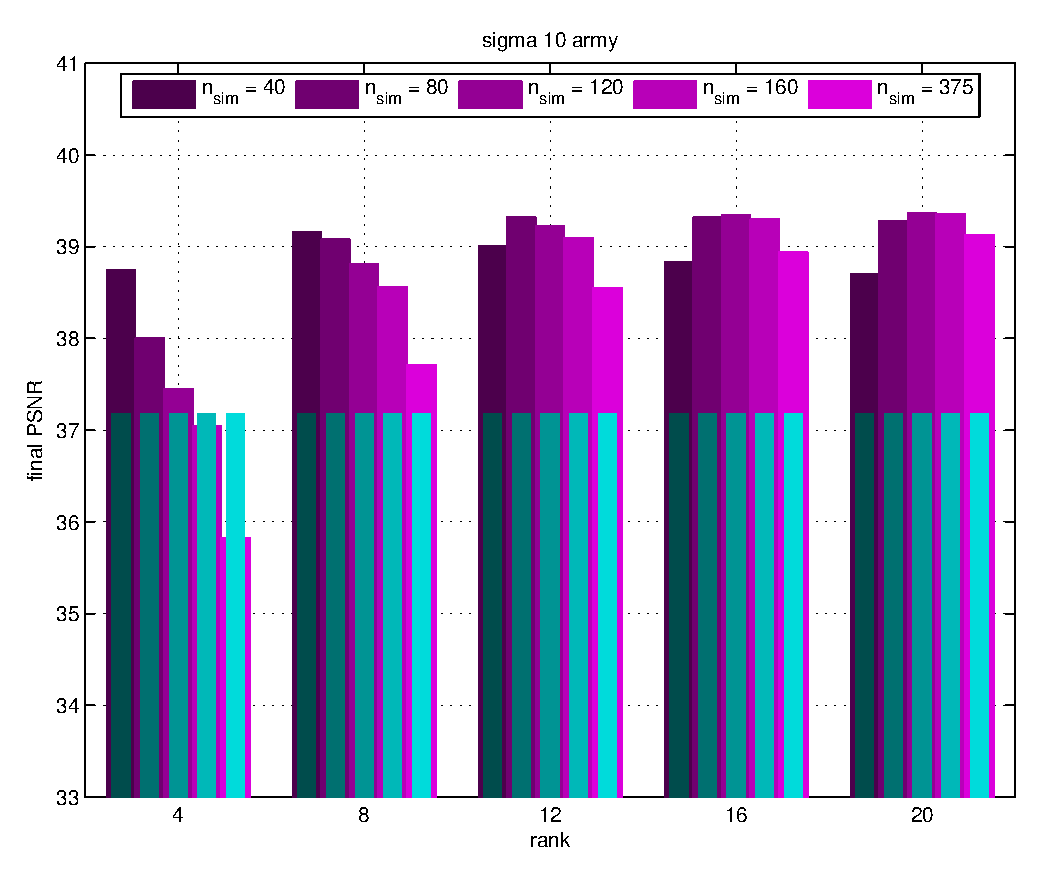
\includegraphics[width=.33\textwidth]{psnr_r2-np2-bars_s10_army.eps}%
		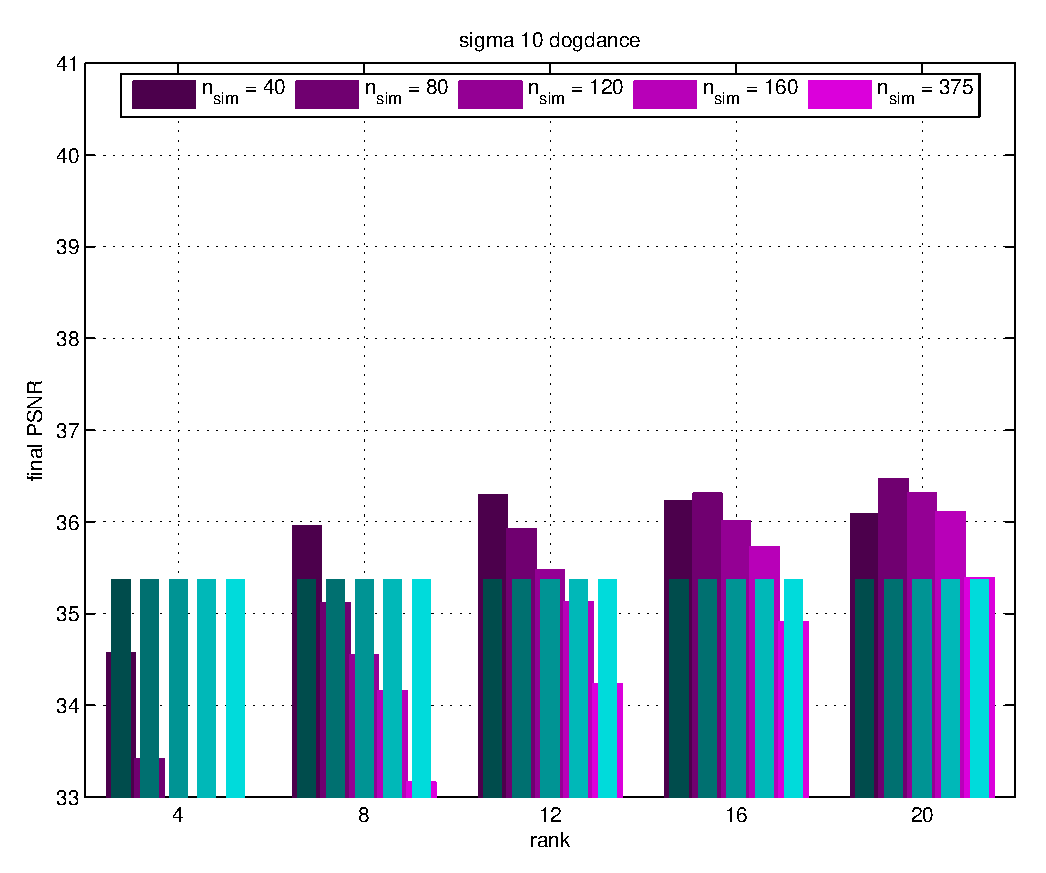
\includegraphics[width=.33\textwidth]{psnr_r2-np2-bars_s10_dogdance.eps}%
		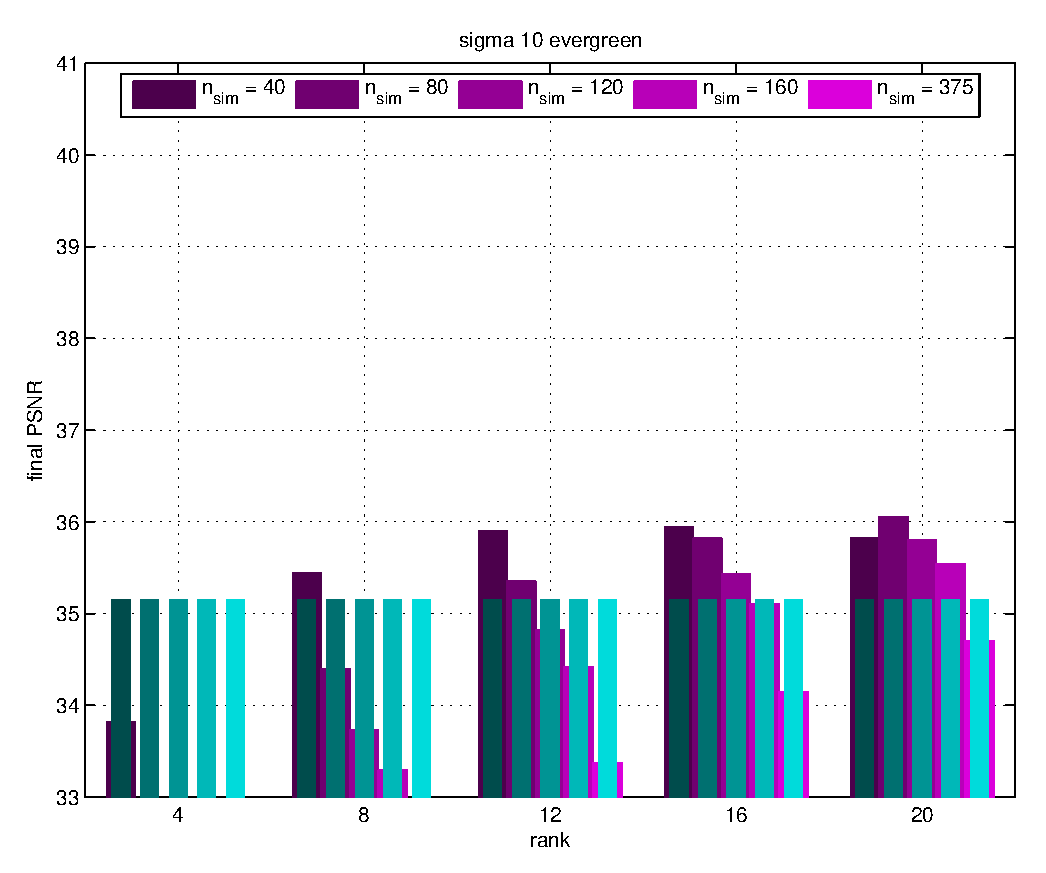
\includegraphics[width=.33\textwidth]{psnr_r2-np2-bars_s10_evergreen.eps}\\
		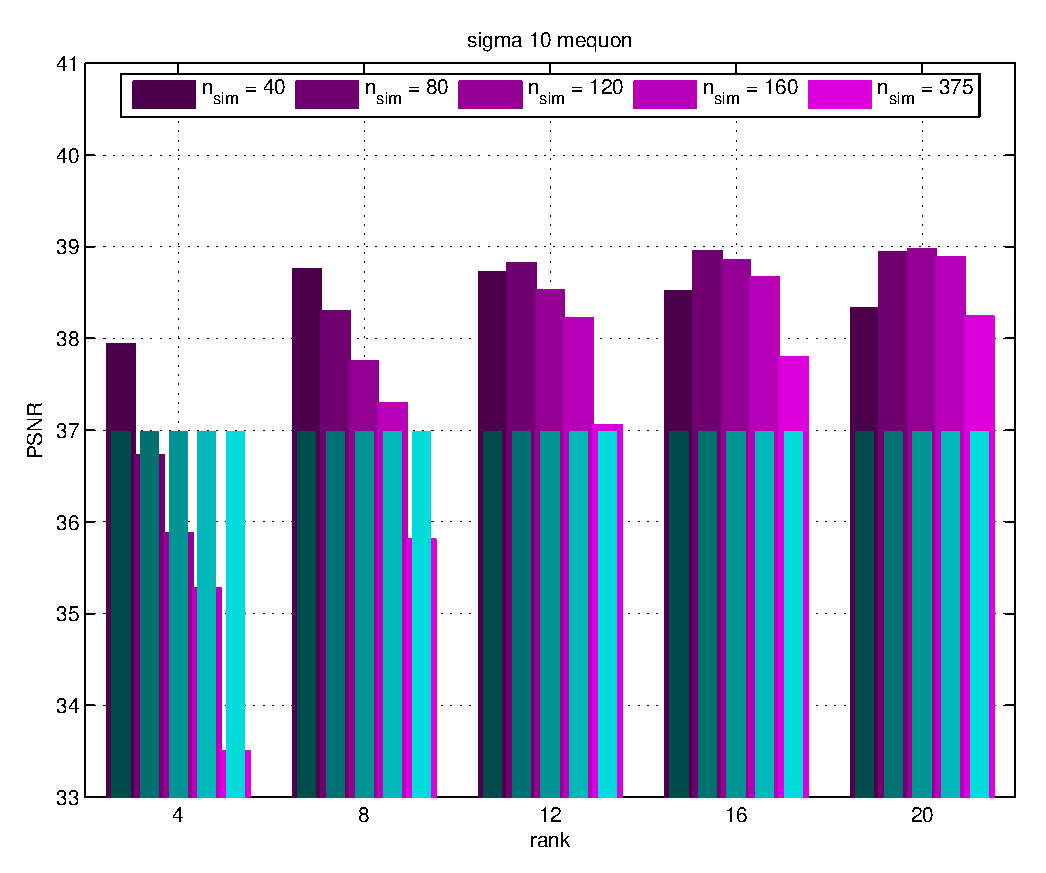
\includegraphics[width=.33\textwidth]{psnr_r2-np2-bars_s10_mequon.eps}%
		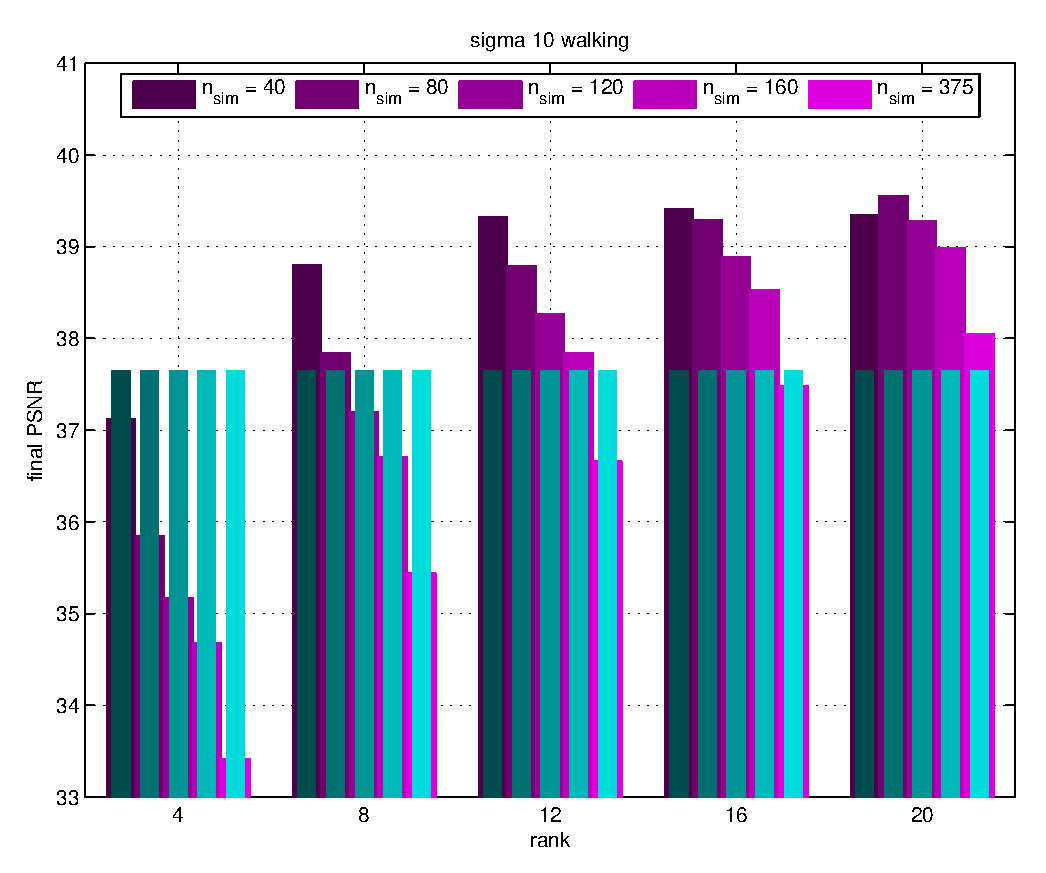
\includegraphics[width=.33\textwidth]{psnr_r2-np2-bars_s10_walking.eps}
	\end{center}

\end{frame}

\begin{frame}{PSNR tables - rank vs. number of patches, stage 2}

	\begin{center}
		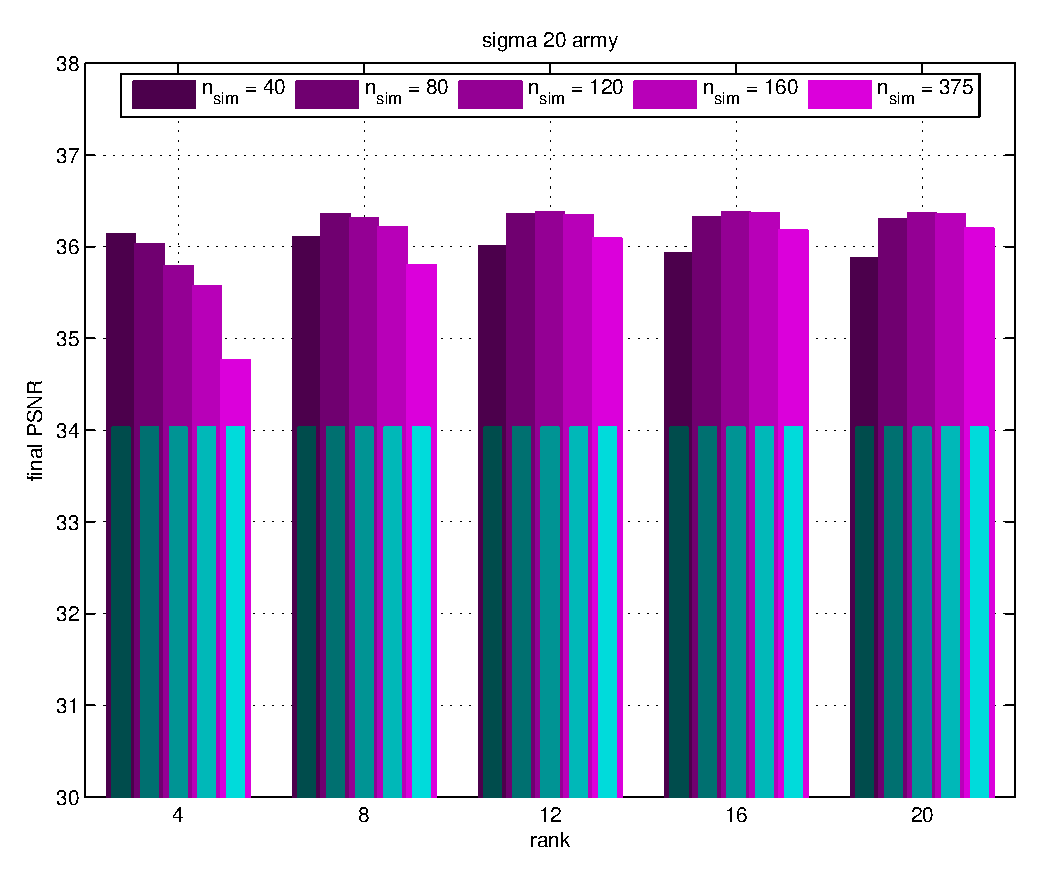
\includegraphics[width=.33\textwidth]{psnr_r2-np2-bars_s20_army.eps}%
		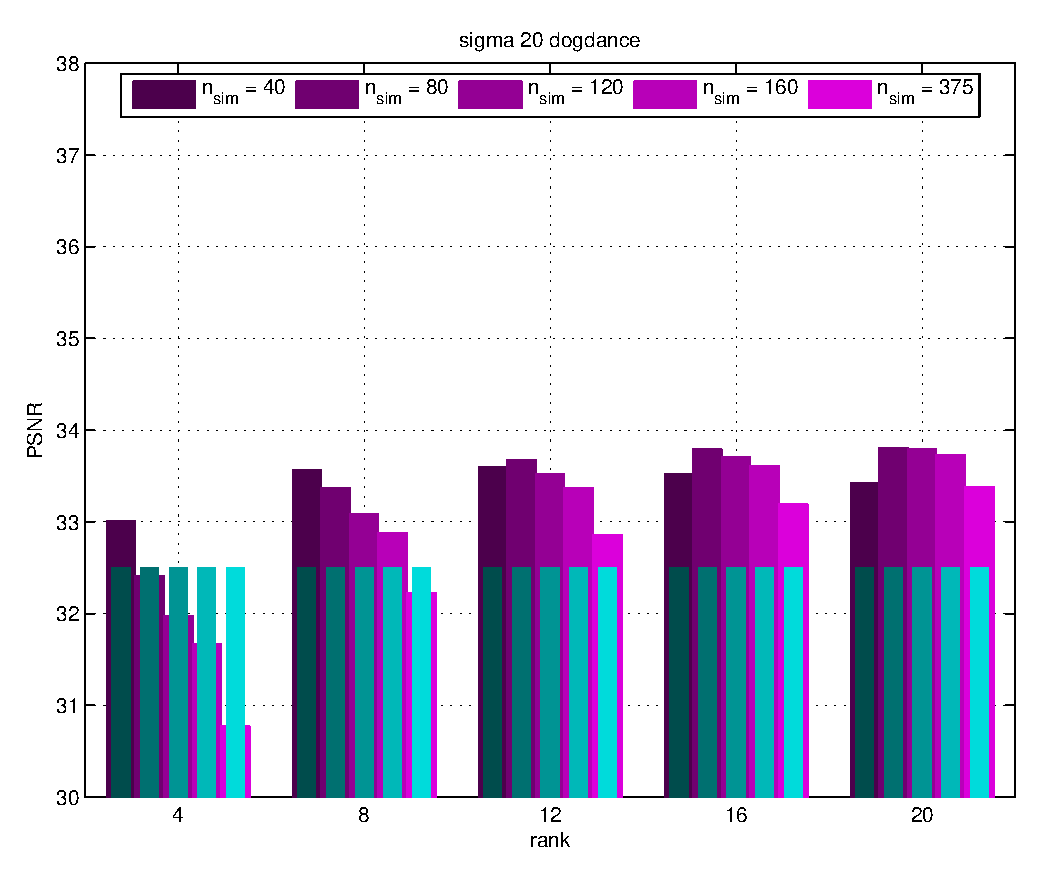
\includegraphics[width=.33\textwidth]{psnr_r2-np2-bars_s20_dogdance.eps}%
		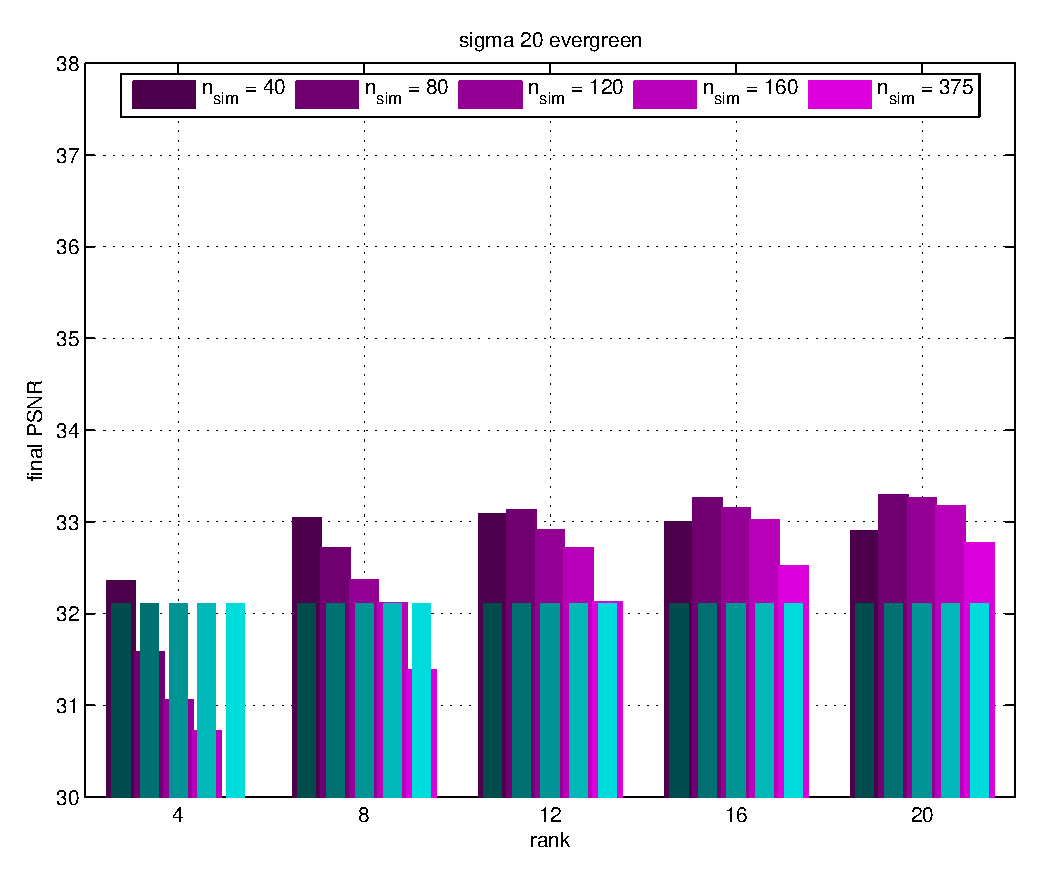
\includegraphics[width=.33\textwidth]{psnr_r2-np2-bars_s20_evergreen.eps}\\
		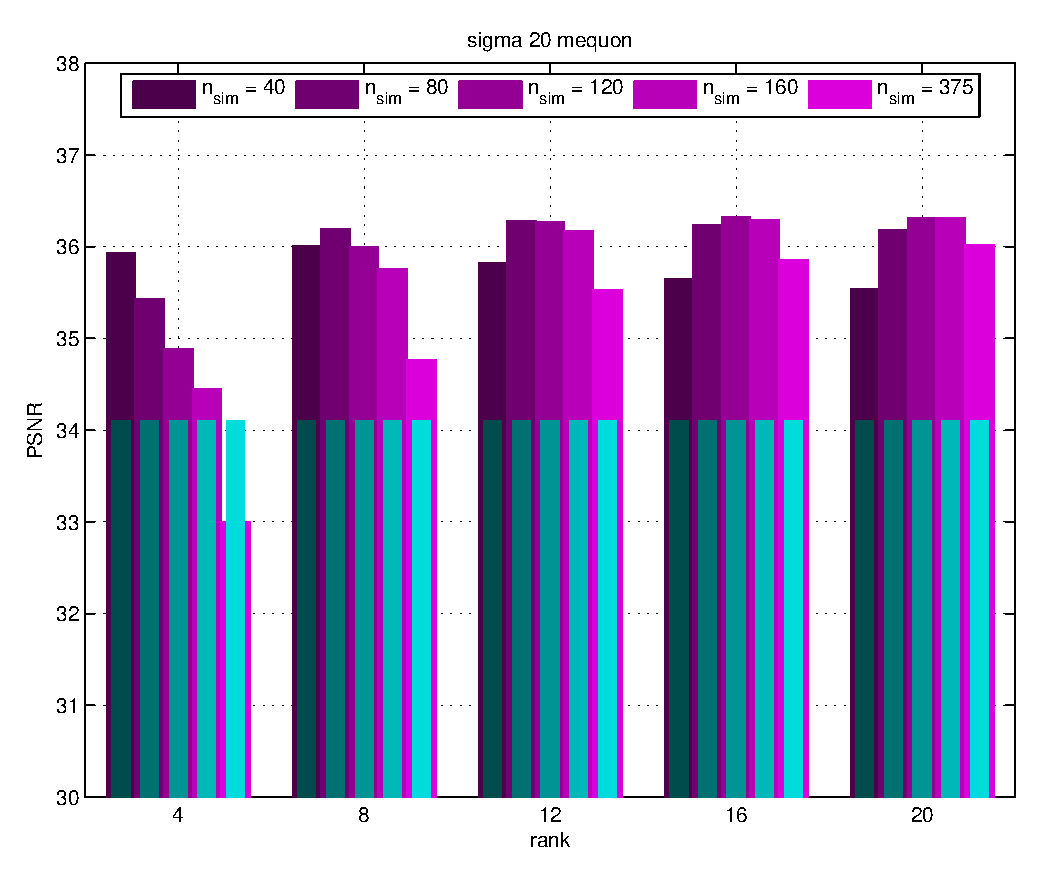
\includegraphics[width=.33\textwidth]{psnr_r2-np2-bars_s20_mequon.eps}%
		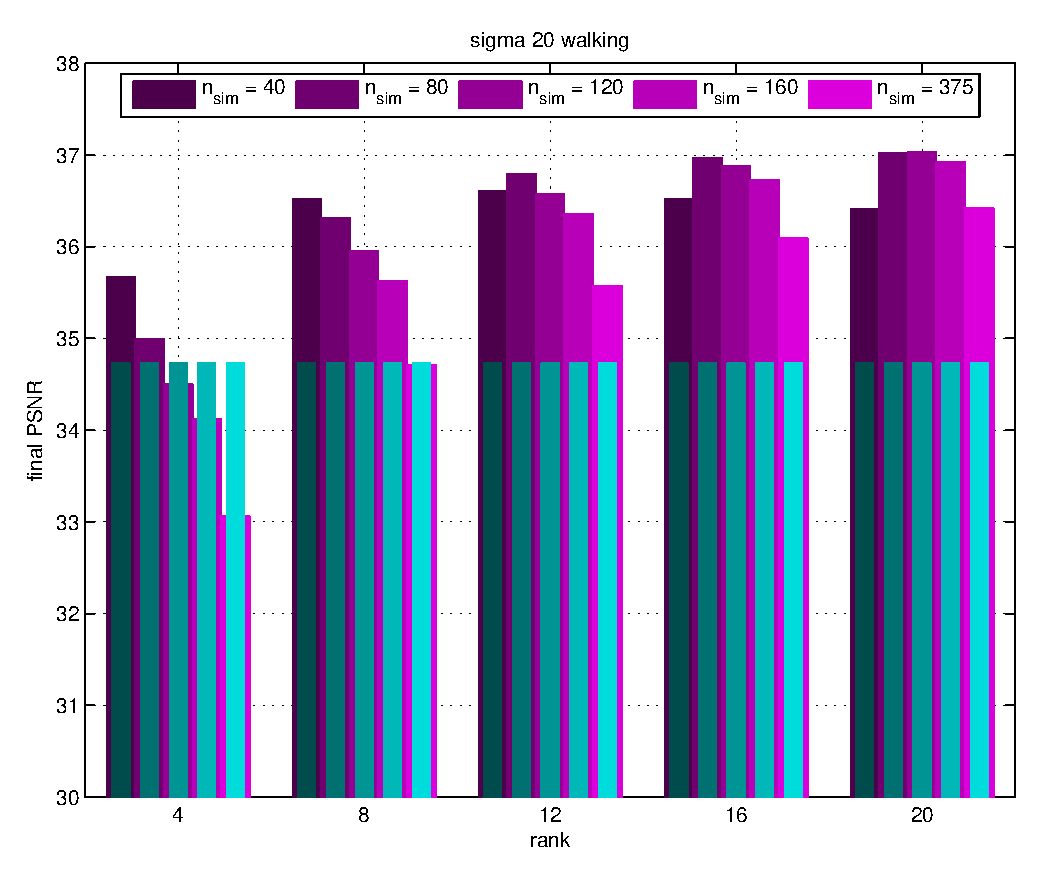
\includegraphics[width=.33\textwidth]{psnr_r2-np2-bars_s20_walking.eps}
	\end{center}

\end{frame}

\begin{frame}{PSNR tables - rank vs. number of patches, stage 2}

	\begin{center}
		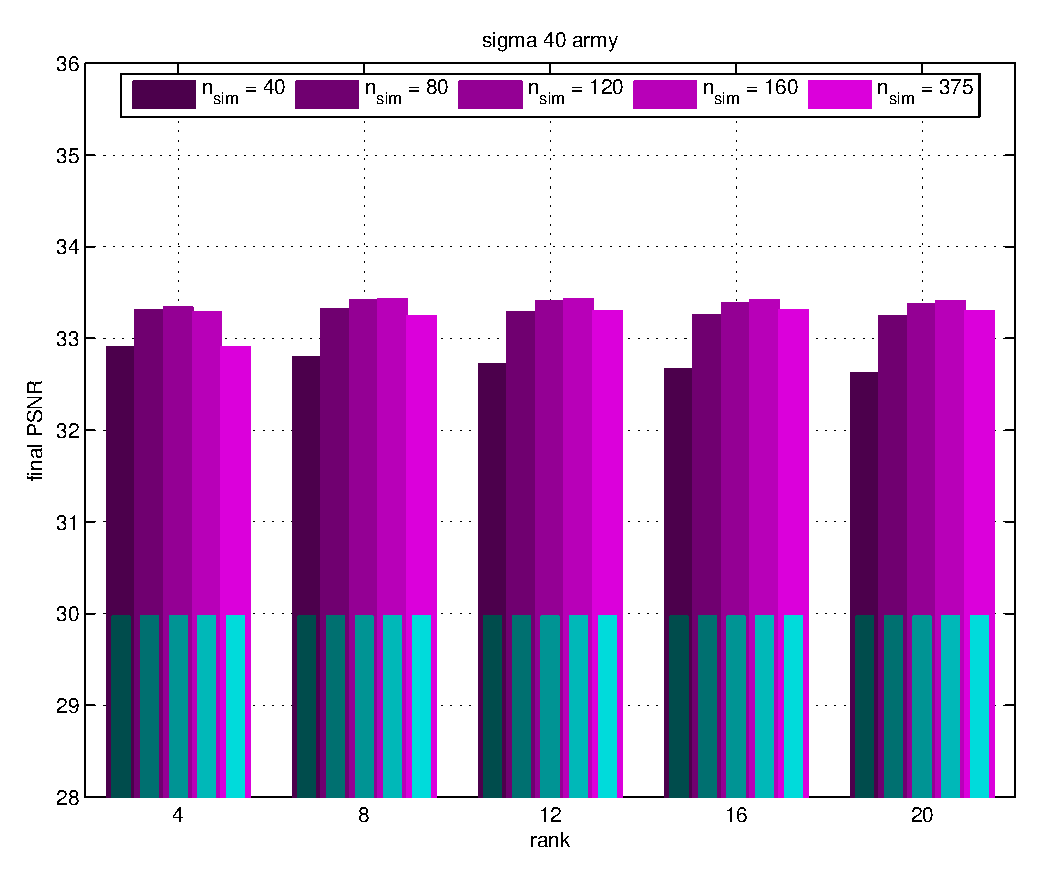
\includegraphics[width=.33\textwidth]{psnr_r2-np2-bars_s40_army.eps}%
		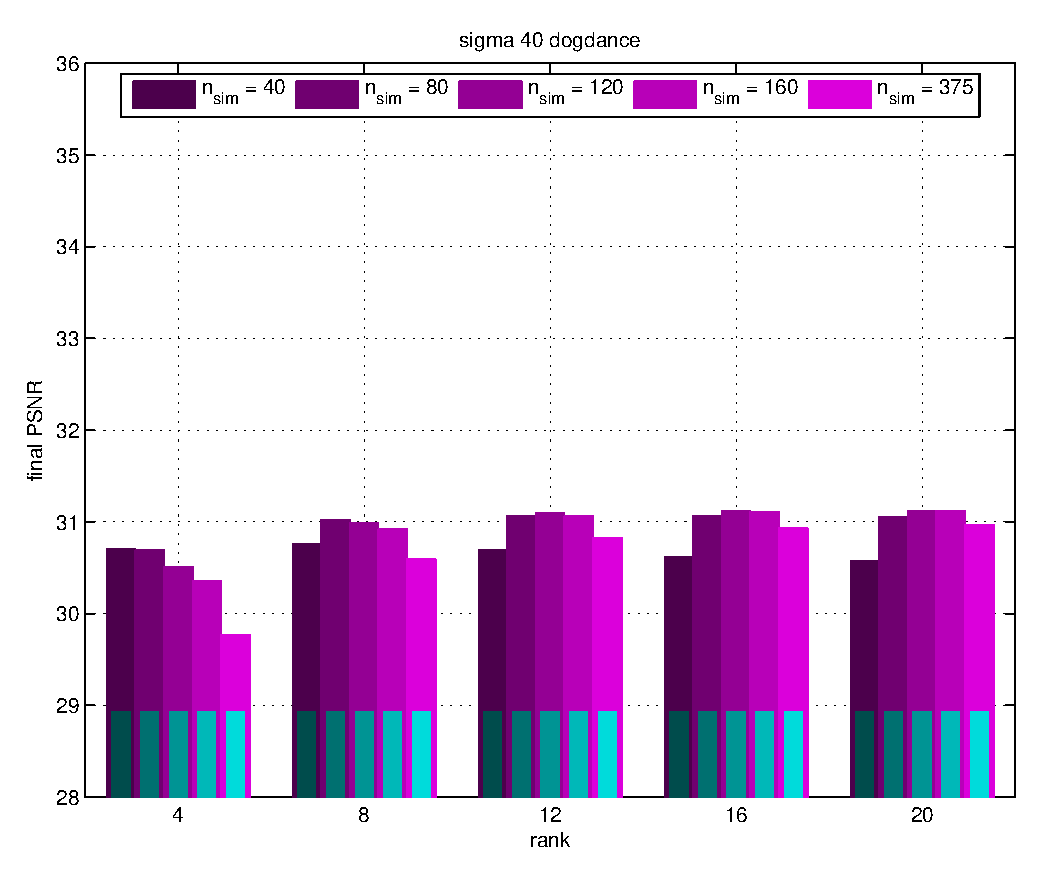
\includegraphics[width=.33\textwidth]{psnr_r2-np2-bars_s40_dogdance.eps}%
		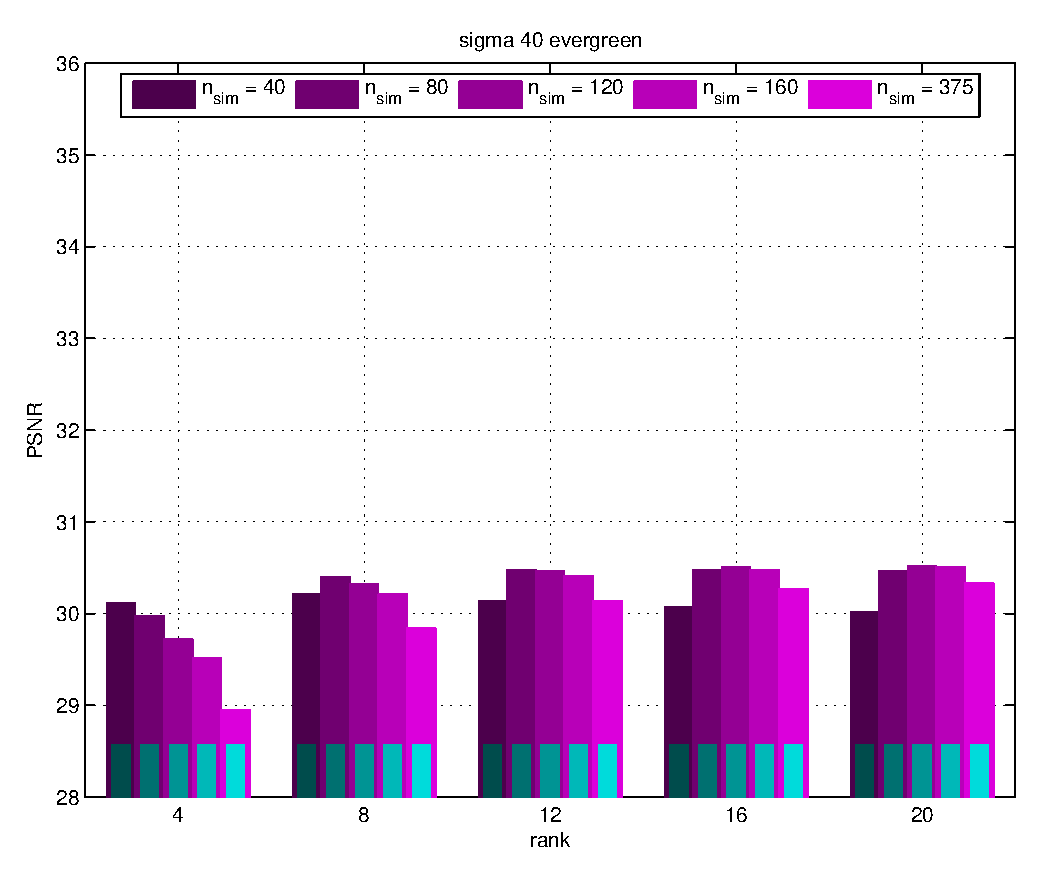
\includegraphics[width=.33\textwidth]{psnr_r2-np2-bars_s40_evergreen.eps}\\
		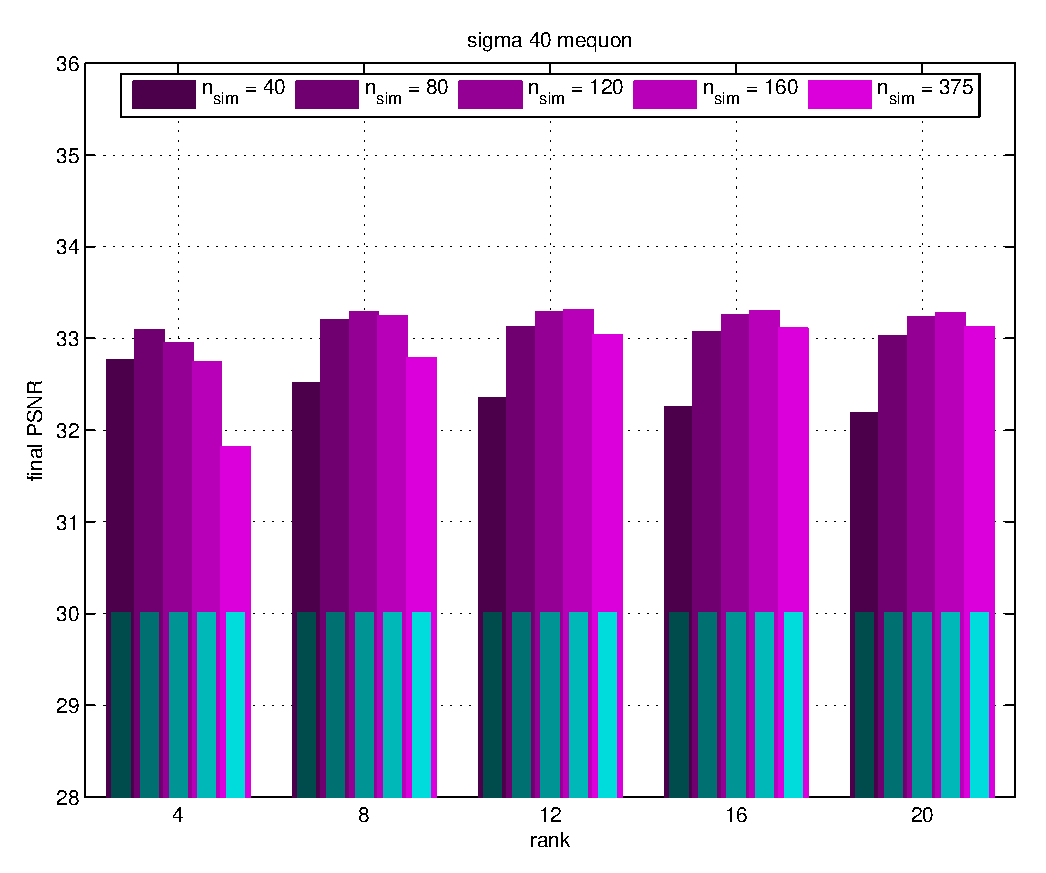
\includegraphics[width=.33\textwidth]{psnr_r2-np2-bars_s40_mequon.eps}%
		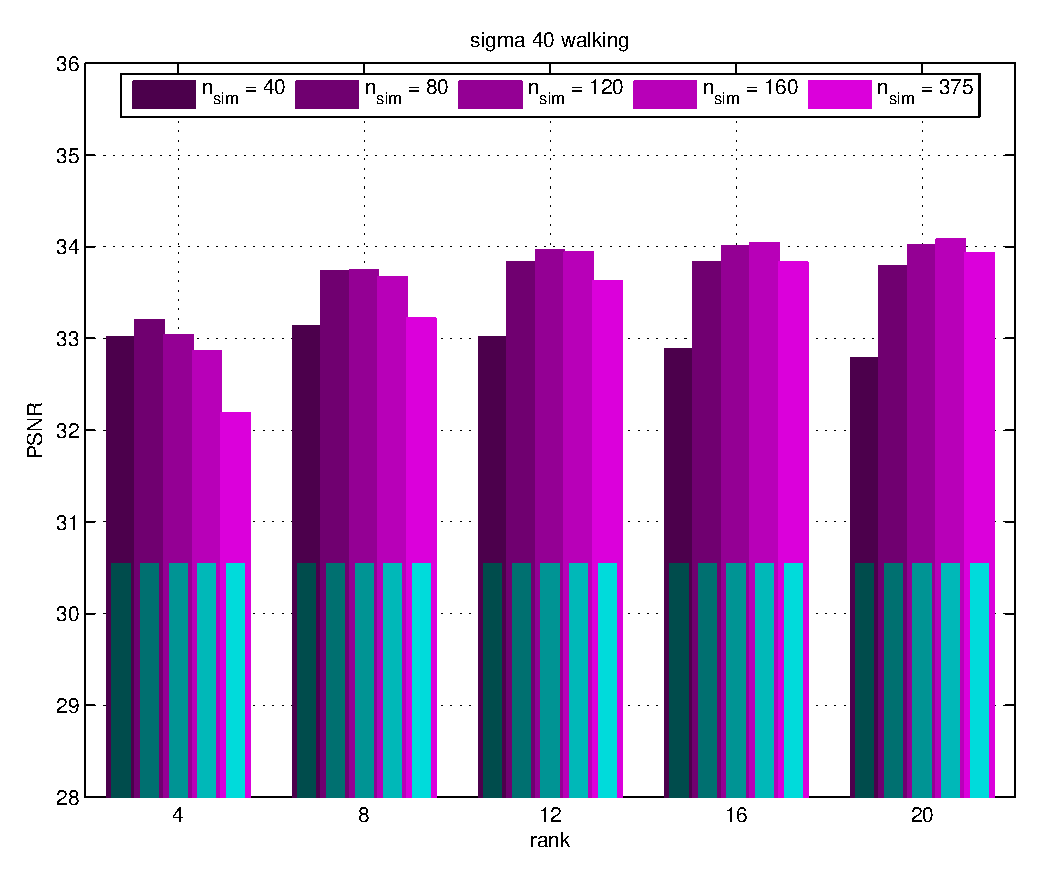
\includegraphics[width=.33\textwidth]{psnr_r2-np2-bars_s40_walking.eps}
	\end{center}

\end{frame}
\restoreframe

\multipleframe
\begin{frame}{Running time tables - rank vs. number of patches, stage 2}

	\begin{center}
		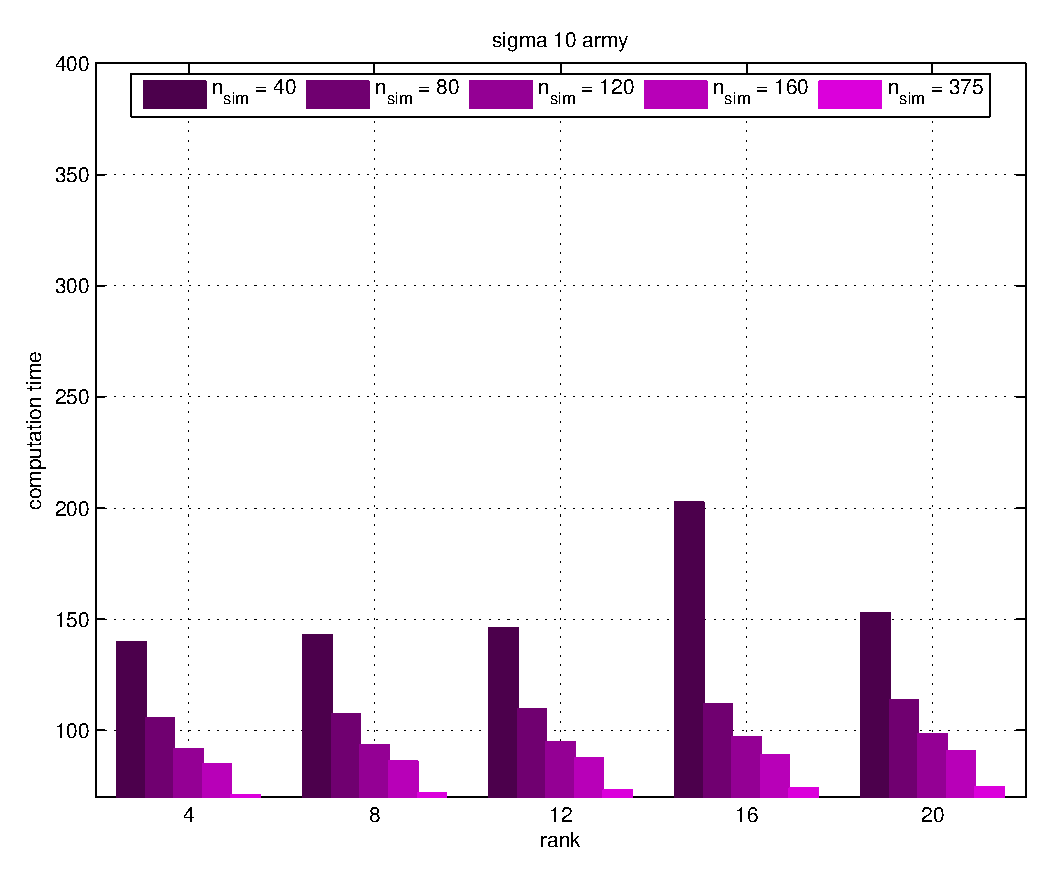
\includegraphics[width=.33\textwidth]{time_r2-np2-bars_s10_army.eps}%
		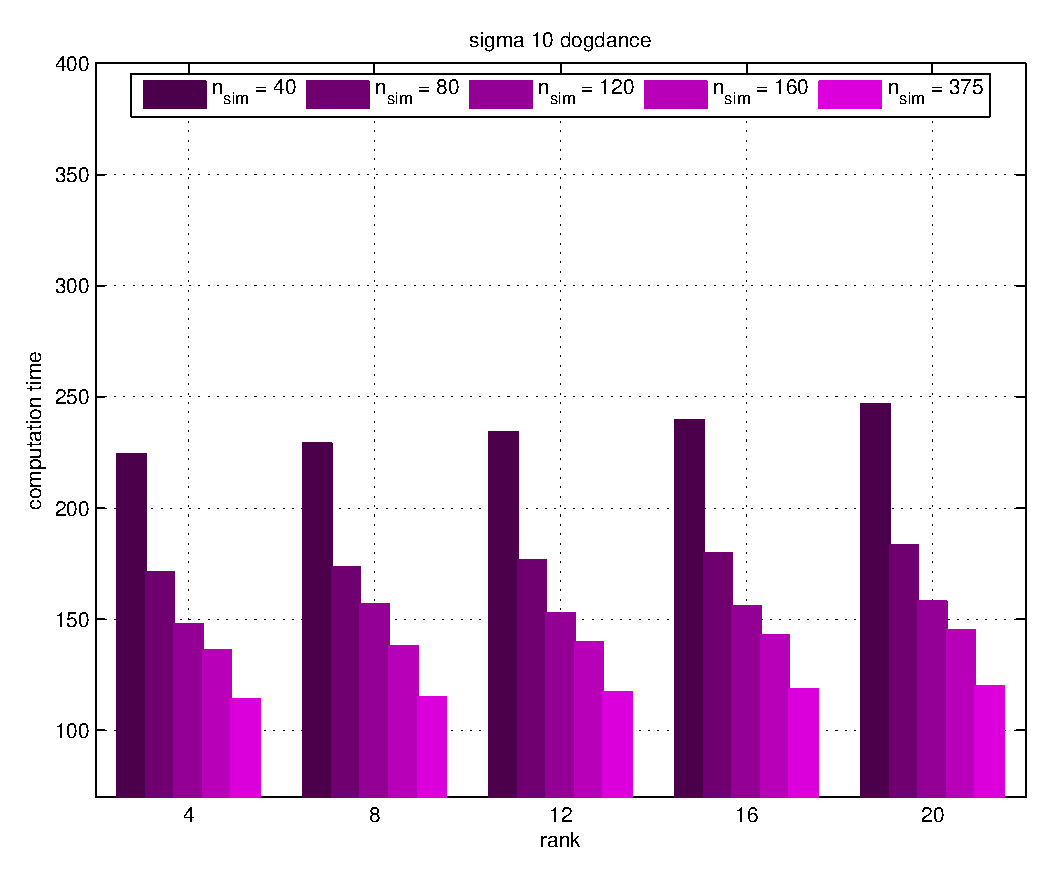
\includegraphics[width=.33\textwidth]{time_r2-np2-bars_s10_dogdance.eps}%
		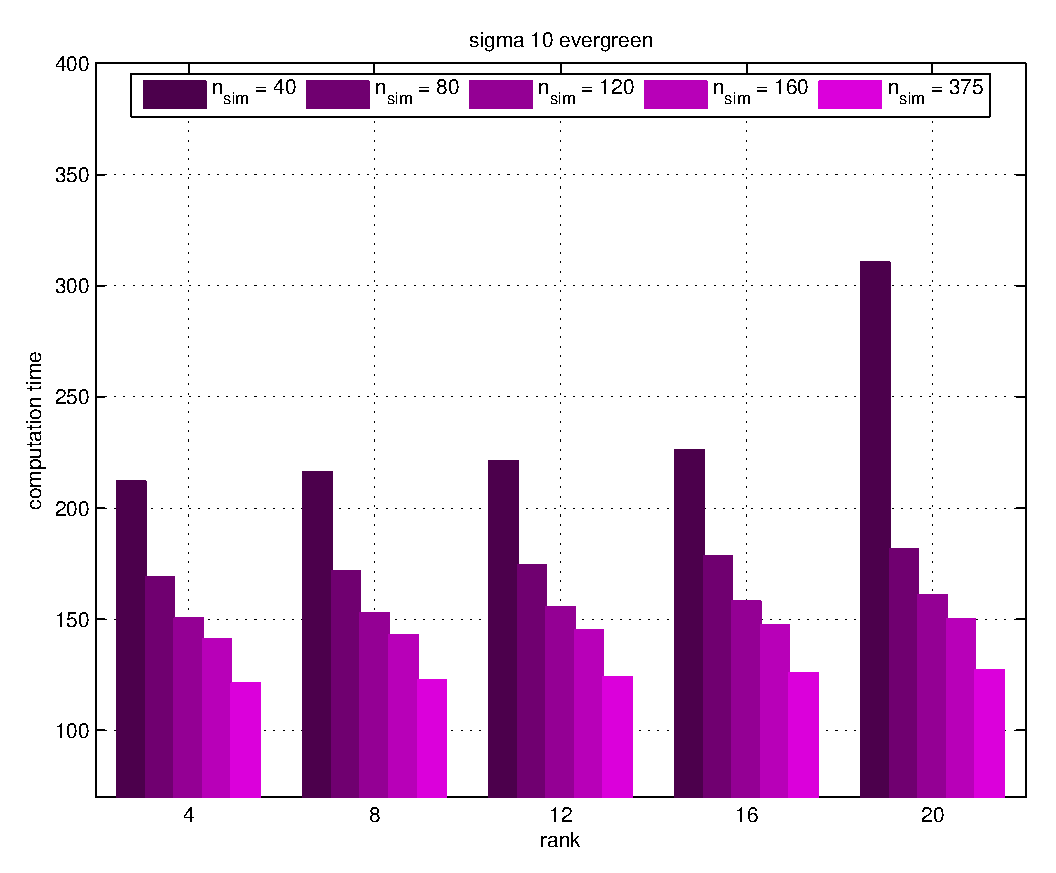
\includegraphics[width=.33\textwidth]{time_r2-np2-bars_s10_evergreen.eps}\\
		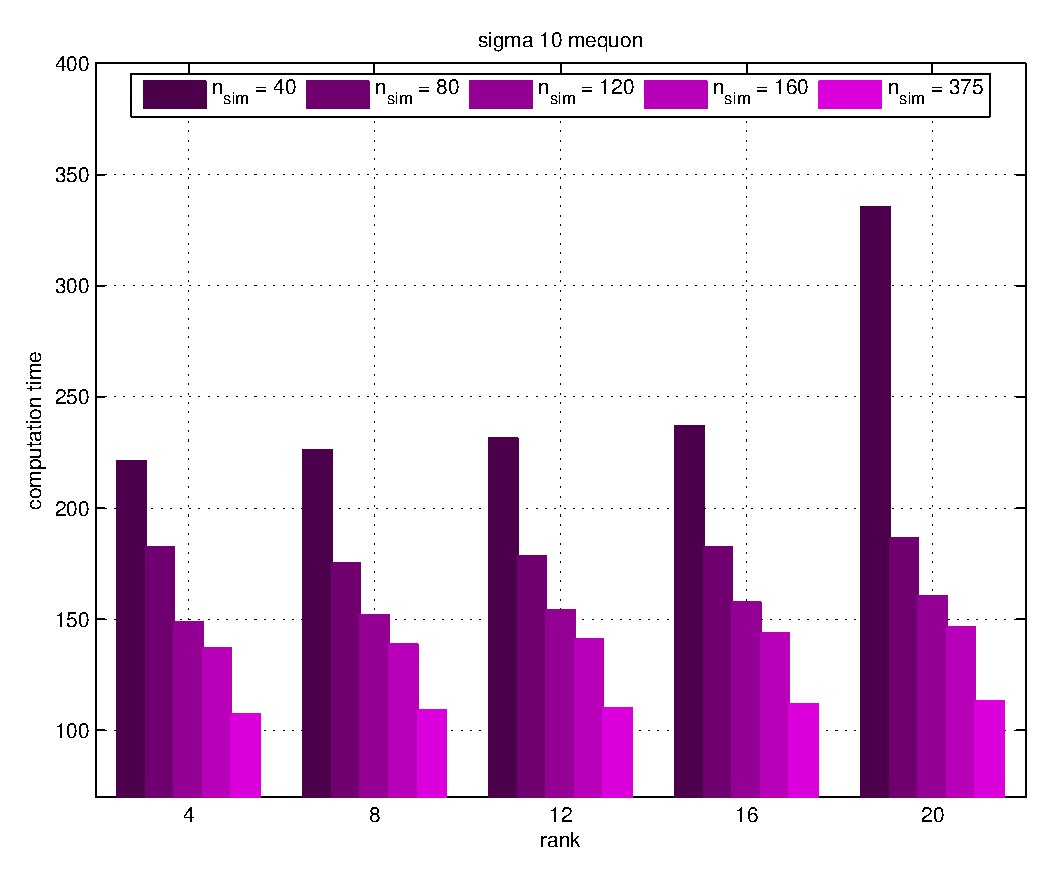
\includegraphics[width=.33\textwidth]{time_r2-np2-bars_s10_mequon.eps}%
		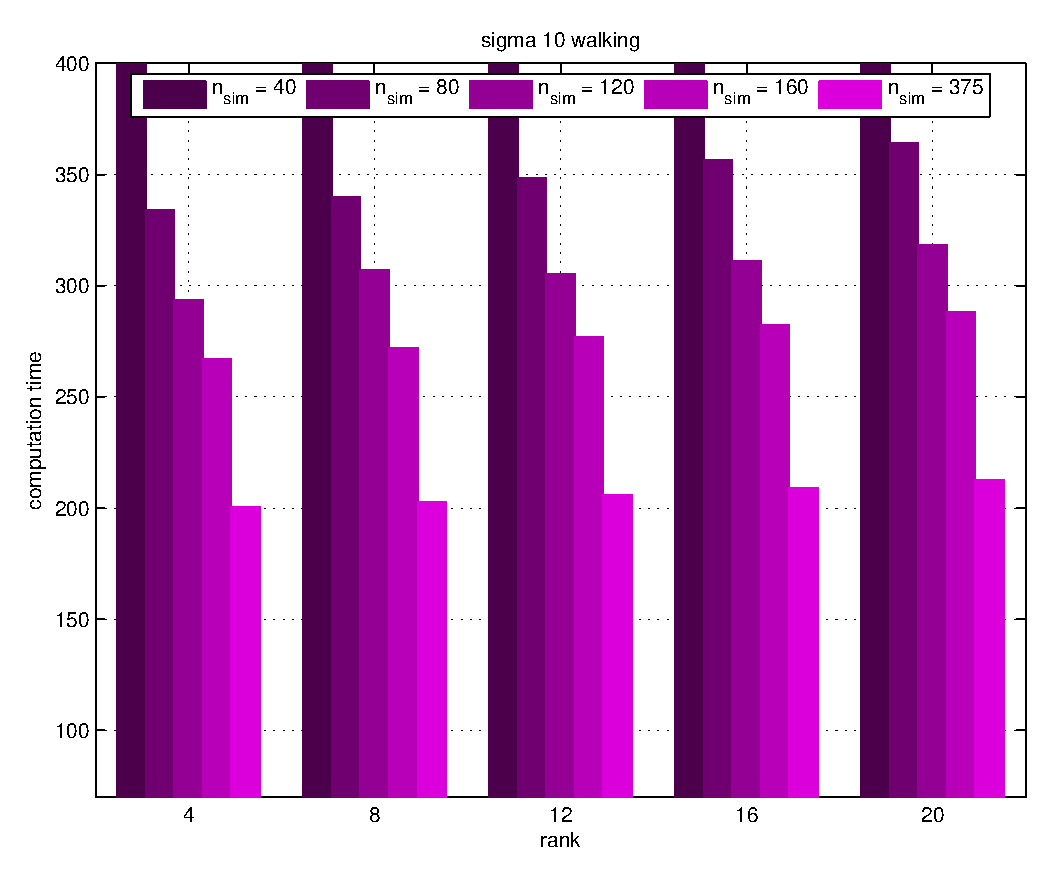
\includegraphics[width=.33\textwidth]{time_r2-np2-bars_s10_walking.eps}
	\end{center}

\end{frame}

\begin{frame}{Running time tables - rank vs. number of patches, stage 2}

	\begin{center}
		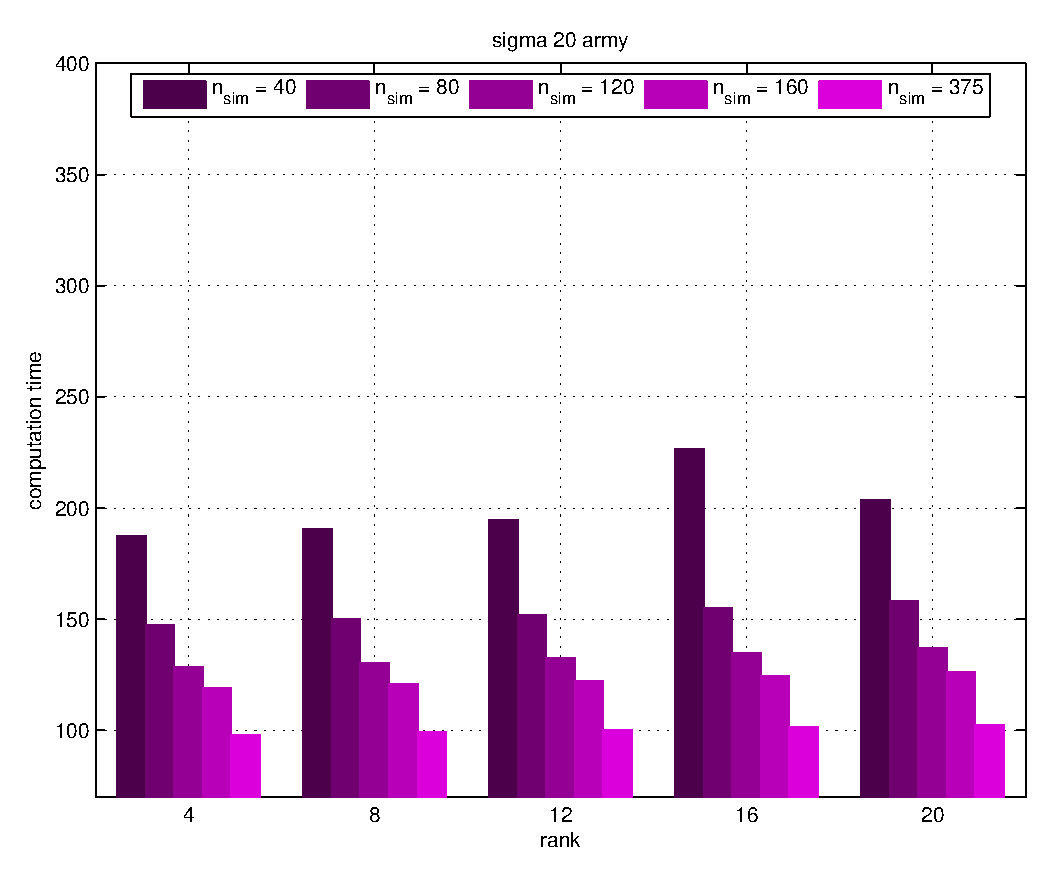
\includegraphics[width=.33\textwidth]{time_r2-np2-bars_s20_army.eps}%
		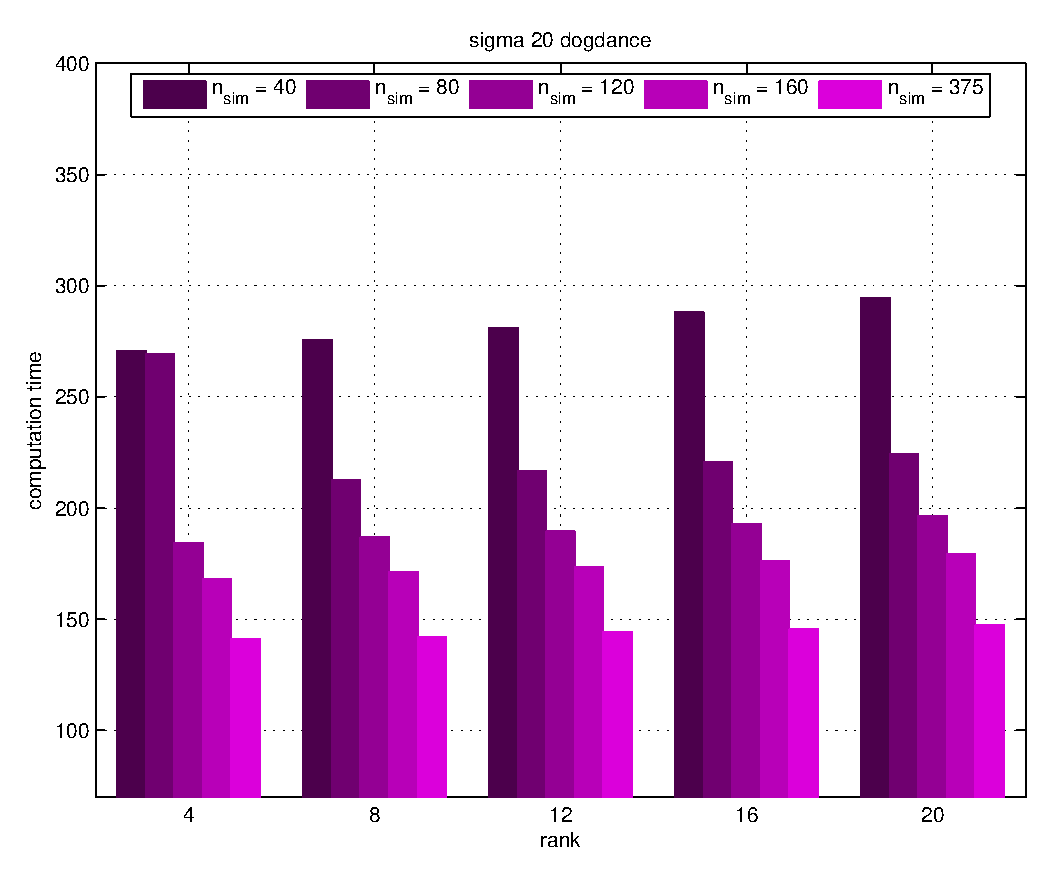
\includegraphics[width=.33\textwidth]{time_r2-np2-bars_s20_dogdance.eps}%
		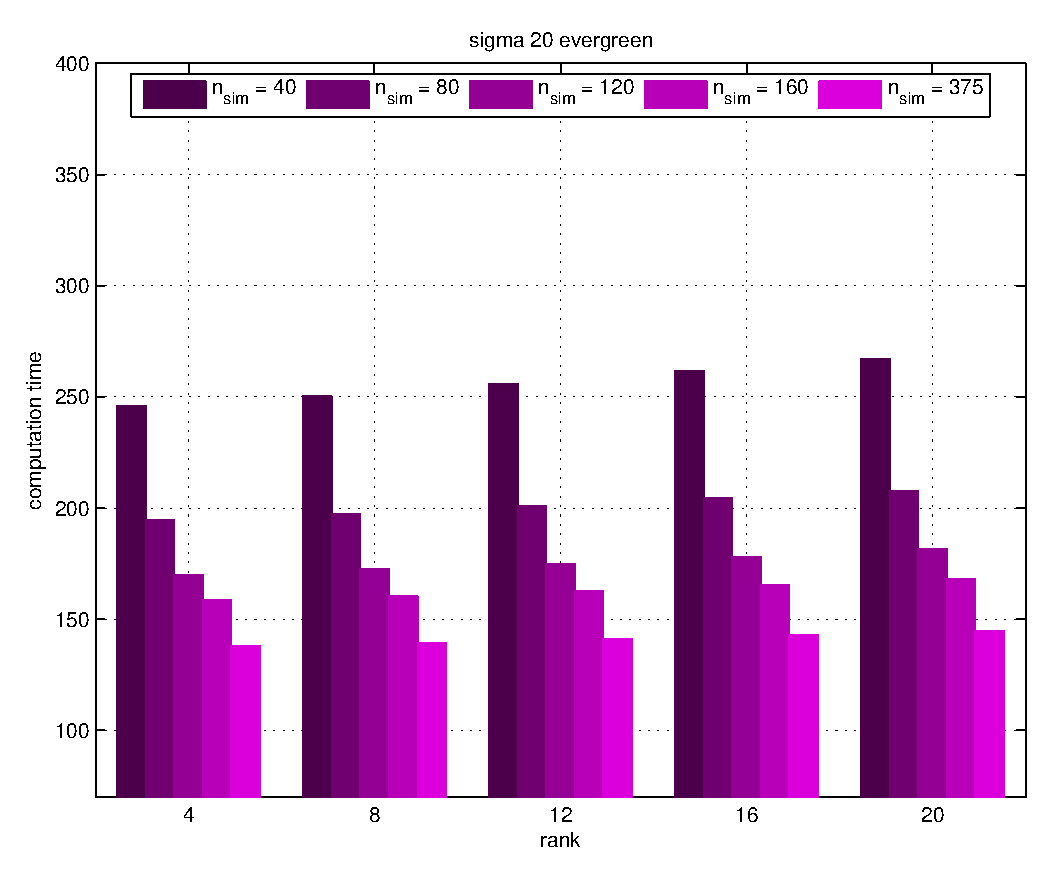
\includegraphics[width=.33\textwidth]{time_r2-np2-bars_s20_evergreen.eps}\\
		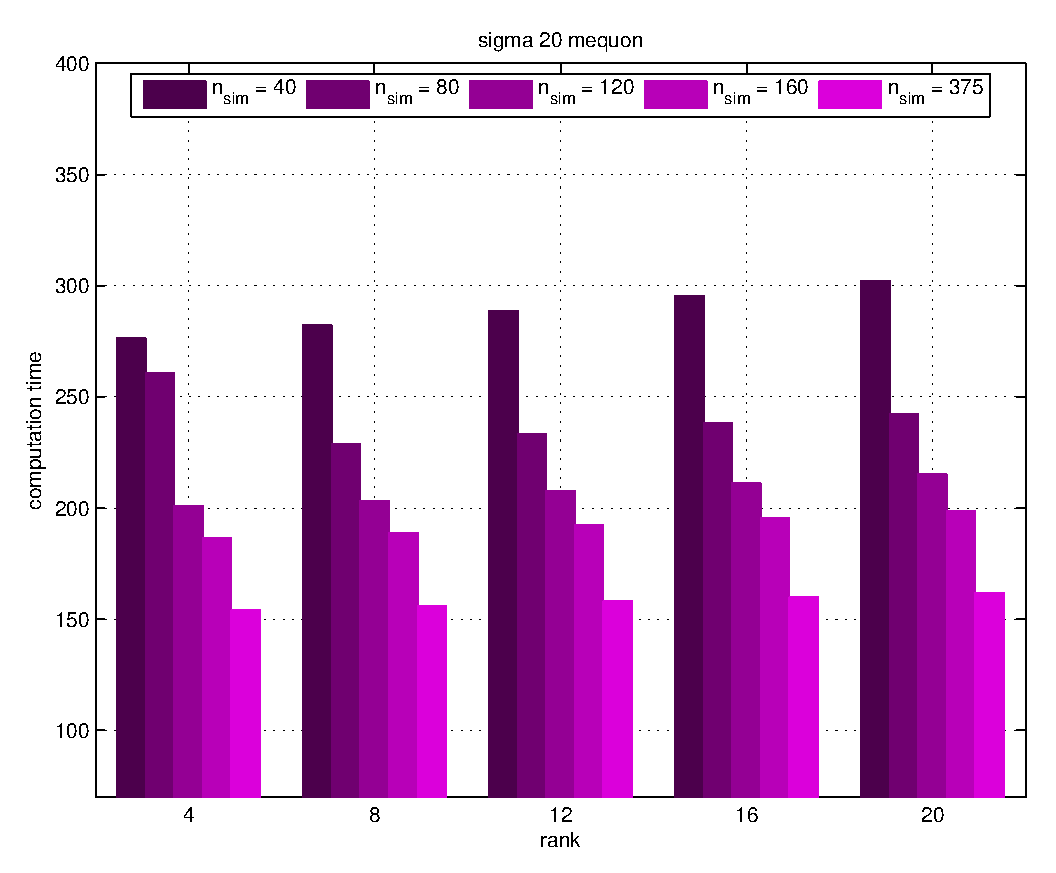
\includegraphics[width=.33\textwidth]{time_r2-np2-bars_s20_mequon.eps}%
		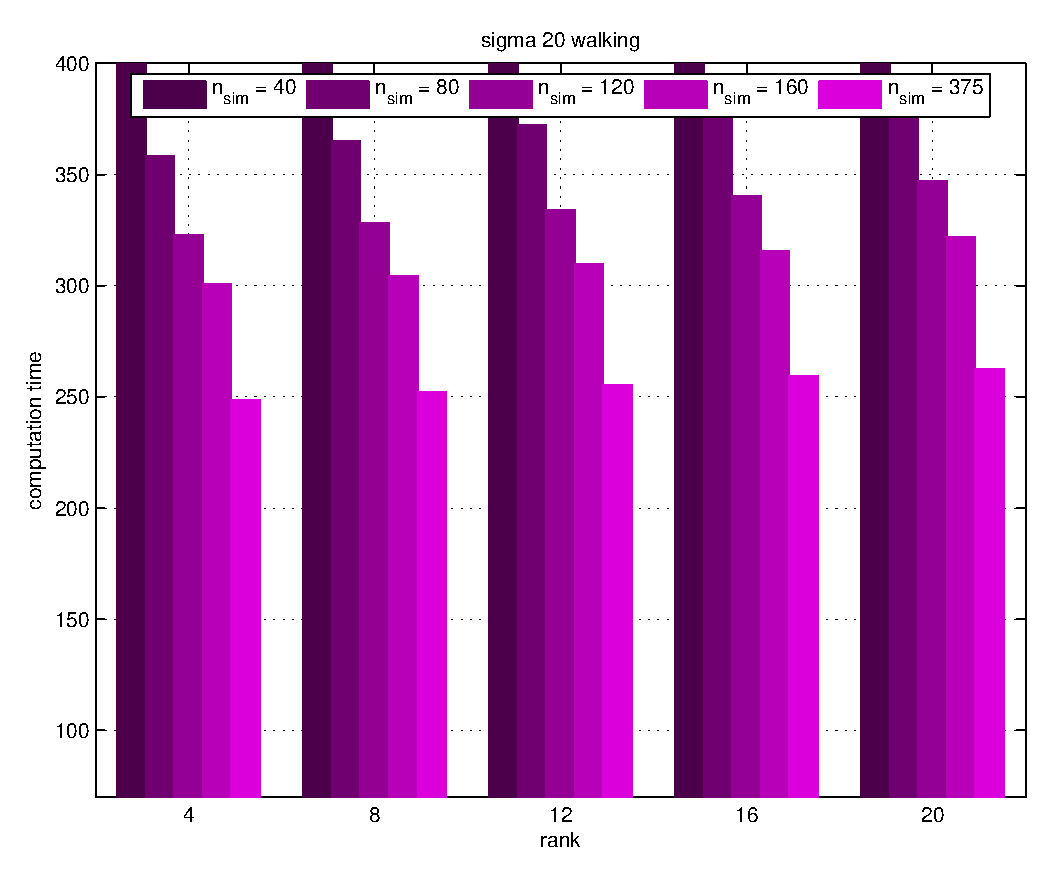
\includegraphics[width=.33\textwidth]{time_r2-np2-bars_s20_walking.eps}
	\end{center}

\end{frame}

\begin{frame}{Running time tables - rank vs. number of patches, stage 2}

	\begin{center}
		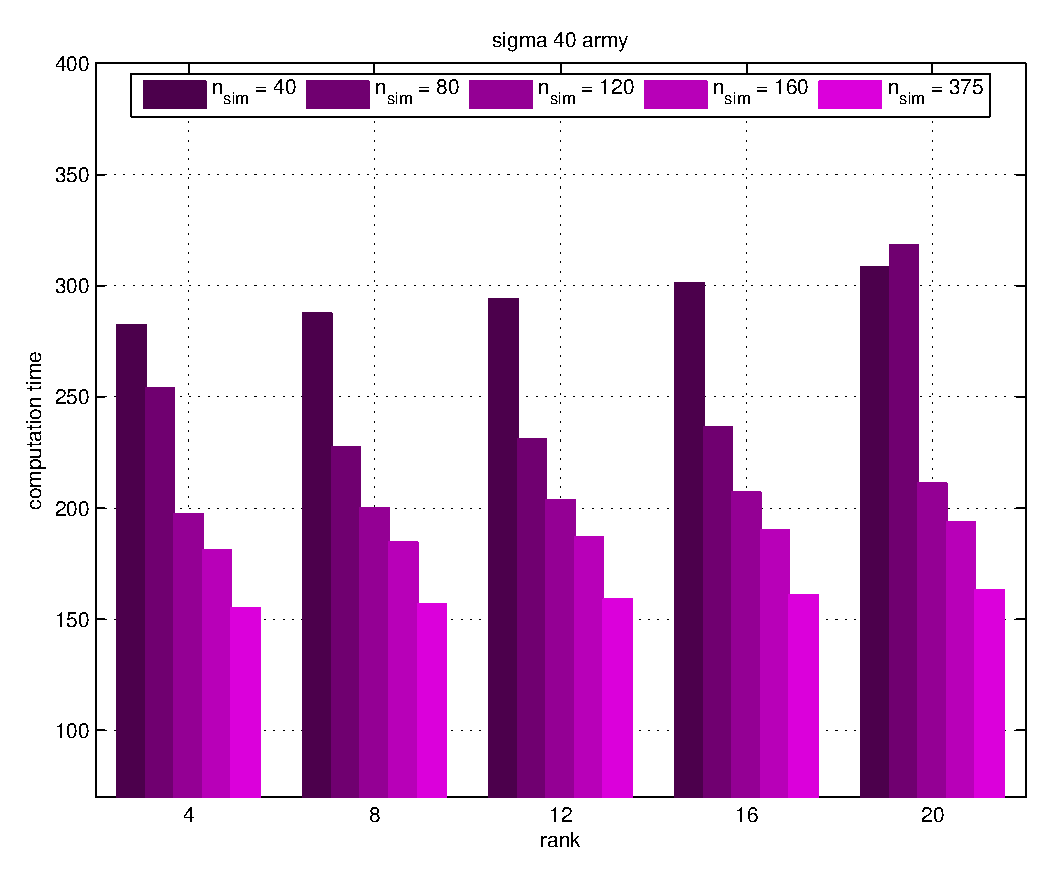
\includegraphics[width=.33\textwidth]{time_r2-np2-bars_s40_army.eps}%
		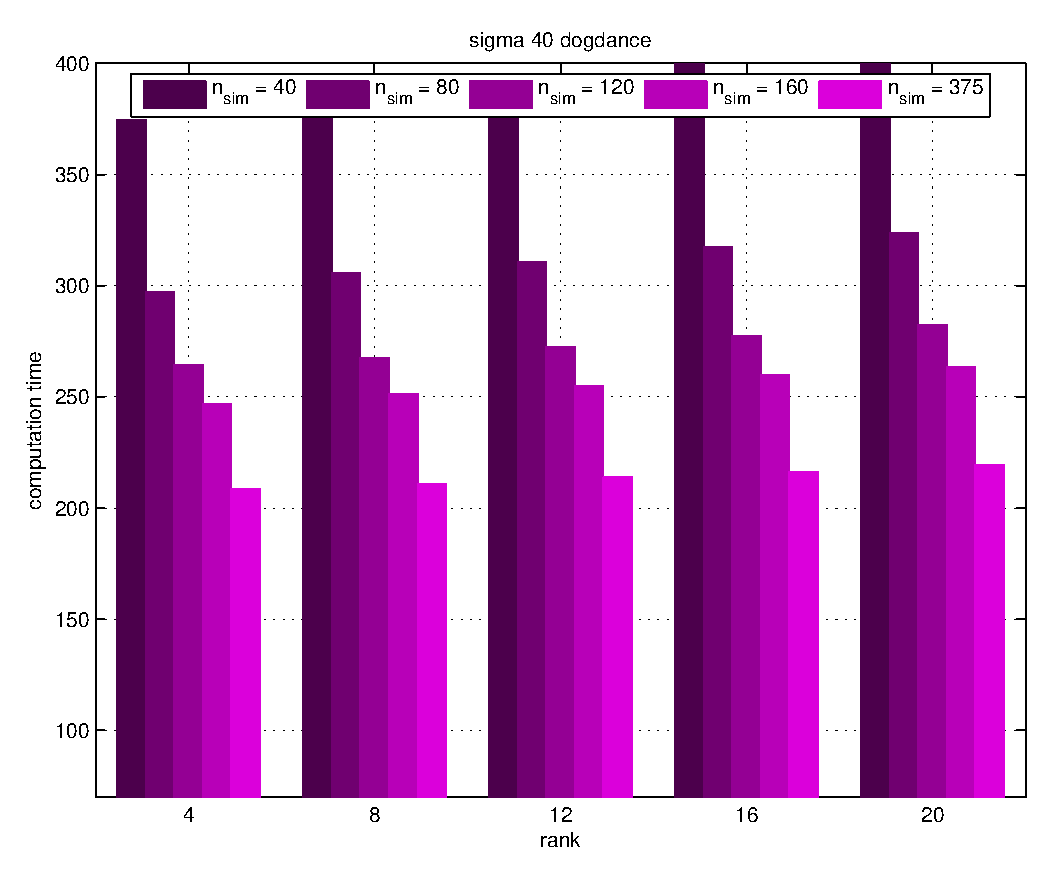
\includegraphics[width=.33\textwidth]{time_r2-np2-bars_s40_dogdance.eps}%
		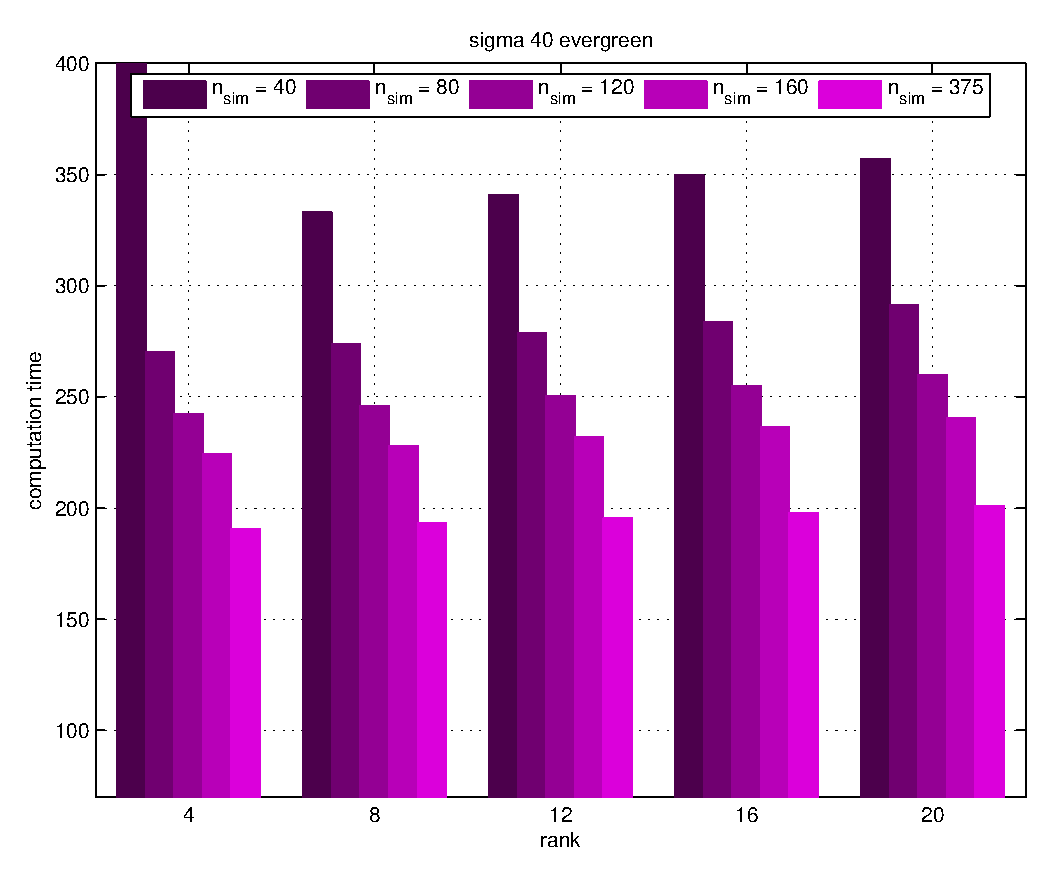
\includegraphics[width=.33\textwidth]{time_r2-np2-bars_s40_evergreen.eps}\\
		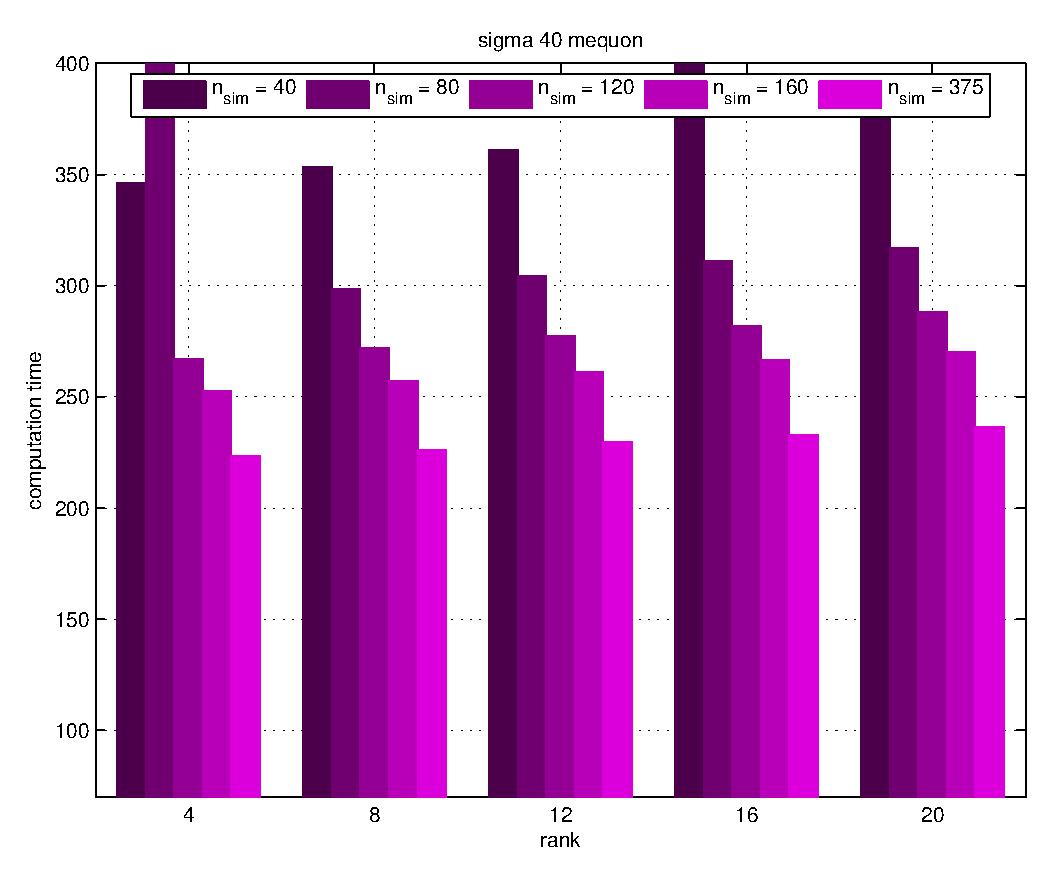
\includegraphics[width=.33\textwidth]{time_r2-np2-bars_s40_mequon.eps}%
		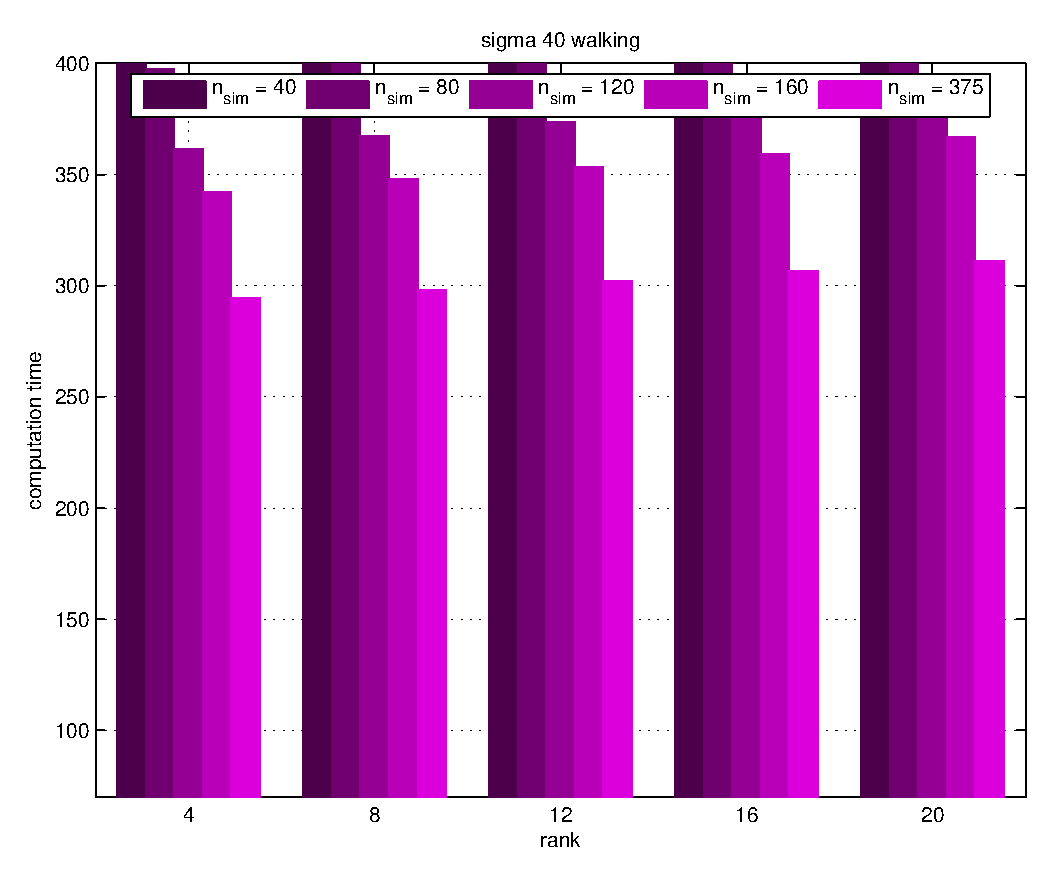
\includegraphics[width=.33\textwidth]{time_r2-np2-bars_s40_walking.eps}
	\end{center}

\end{frame}

\begin{frame}{Conclusions - rank vs. number of patches, stage 2}

	From the preceeding results, we conclude that a good trade-off between PSNR and running time
	is given by:

	\[\text{rank} = 16 \quad\text{ and }\quad n_{\text{sim}} = 160.\]

\end{frame}
\restoreframe

\multipleframe
\begin{frame}{PSNR tables - rank vs. number of patches, stage 1}

	We set the following parameters fixed, and vary the rank and the number of similar
	patches in the second step.

	\begin{center}
	\begin{tabular}{l | c c | c c | c c }
		& \multicolumn{2}{c|}{$\sigma = 10$} 
		& \multicolumn{2}{c|}{$\sigma = 20$} 
		& \multicolumn{2}{c}{$\sigma = 40$} \\
		                            & 1st  & 2nd  & 1st  & 2nd  & 1st  & 2nd \\\hline\hline
		Patch size (spatial)        &  5   &   5  &  5   &   5  &  5   &   5 \\
		Patch size (temporal)       &  4   &   4  &  4   &   4  &  4   &   4 \\
		Number of patches           &      & 160  &      & 160  &      & 160 \\
		Rank of cov. matrix         &      &  16  &      &  16  &      & 16  \\
		Distance threshold $\tau$   & n/a  & 432  & n/a  & 432  & n/a  & 432 \\
		Spatial search window       & 13   & 37   & 37   & 37   & 37   & 37  \\
		Temporal search range       & 5    & 5    & 5    & 5    & 5    & 5   \\\hline
		Beta                        & 1    & 1    & 1    & 1    & 1    & 1   \\\hline
	\end{tabular}
	\end{center}

	\bigskip

	\structure{In the following plots, the values of PSNR for the basic and
		final estimates, obtained with the previous settings for the stage 1 (full
		rank and $n_{\text{sim}} = 375$) are shown by two horizontal dashed
		lines.}

\end{frame}

\begin{frame}{PSNR tables - rank vs. number of patches, stage 1}

	\begin{center}
		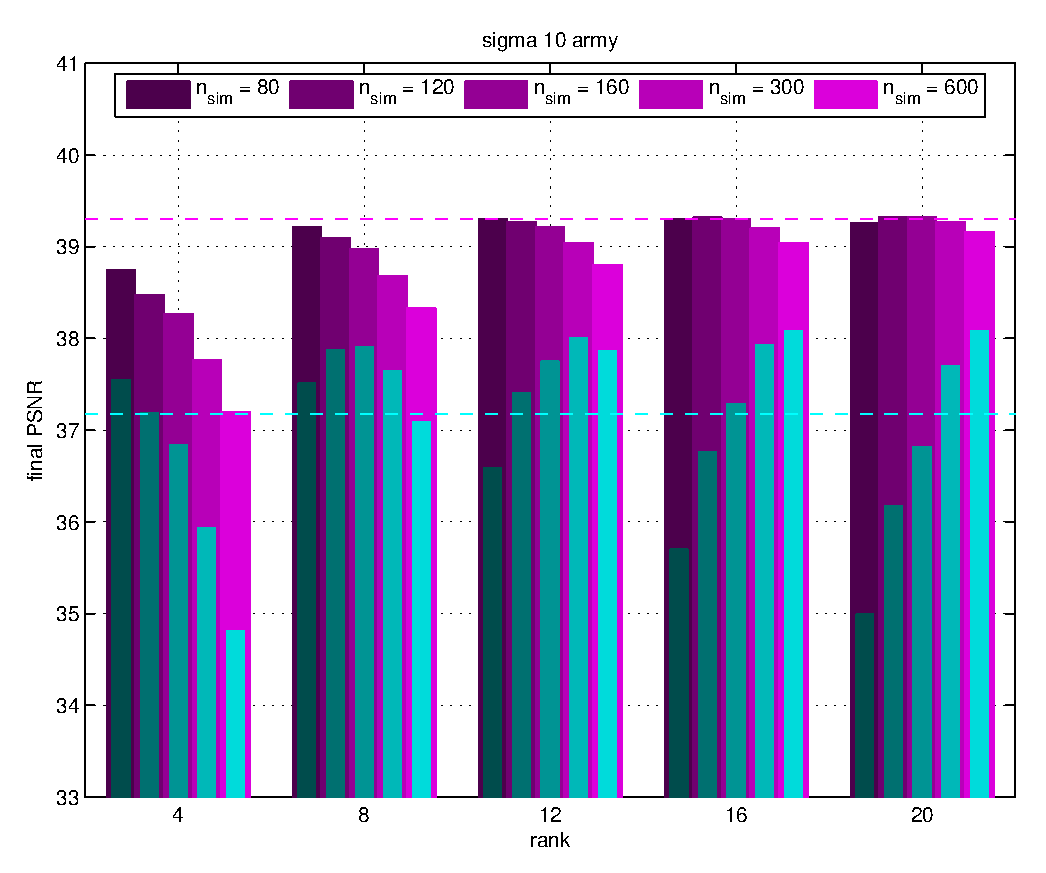
\includegraphics[width=.33\textwidth]{psnr_r1-np1-bars_s10_army.eps}%
		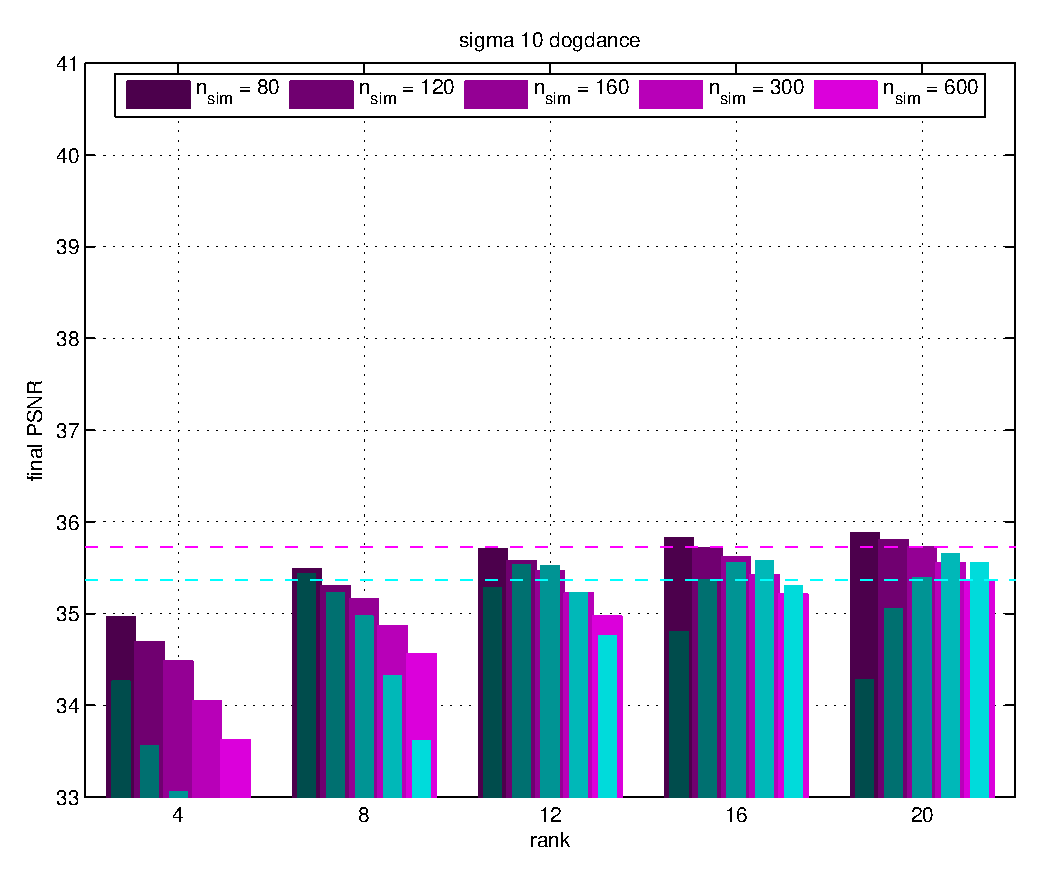
\includegraphics[width=.33\textwidth]{psnr_r1-np1-bars_s10_dogdance.eps}%
		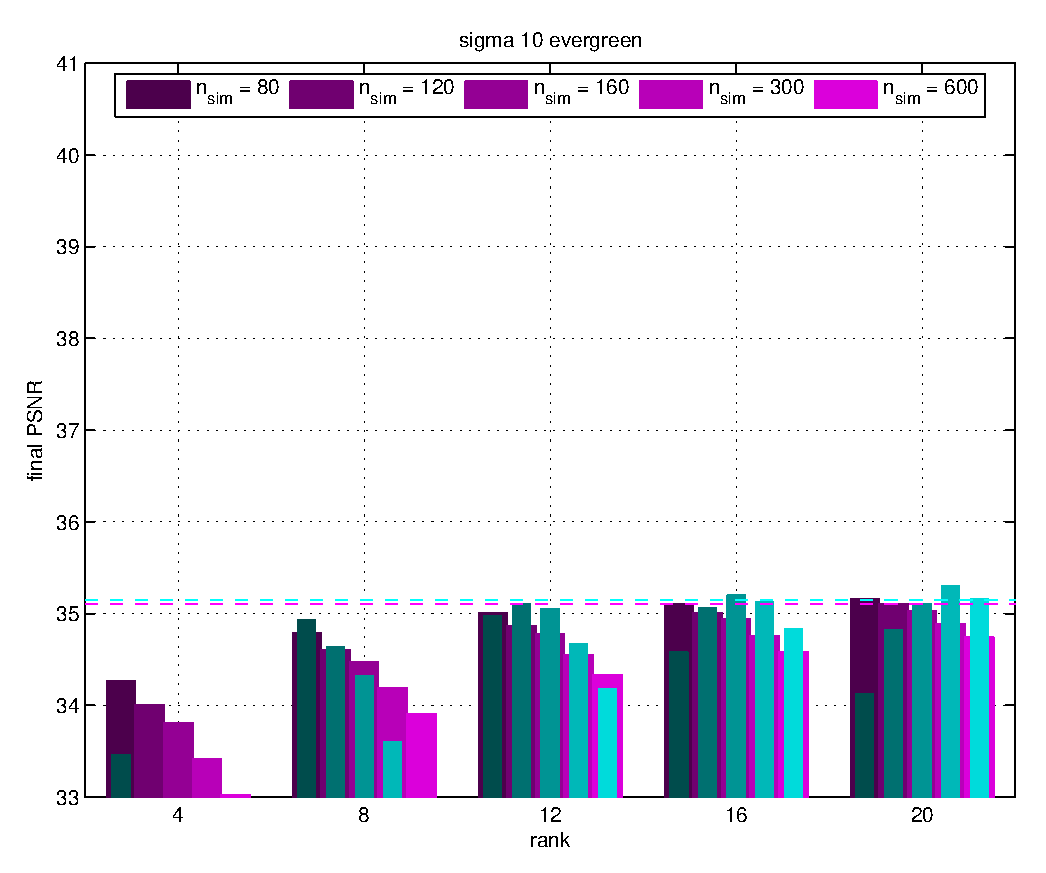
\includegraphics[width=.33\textwidth]{psnr_r1-np1-bars_s10_evergreen.eps}\\
		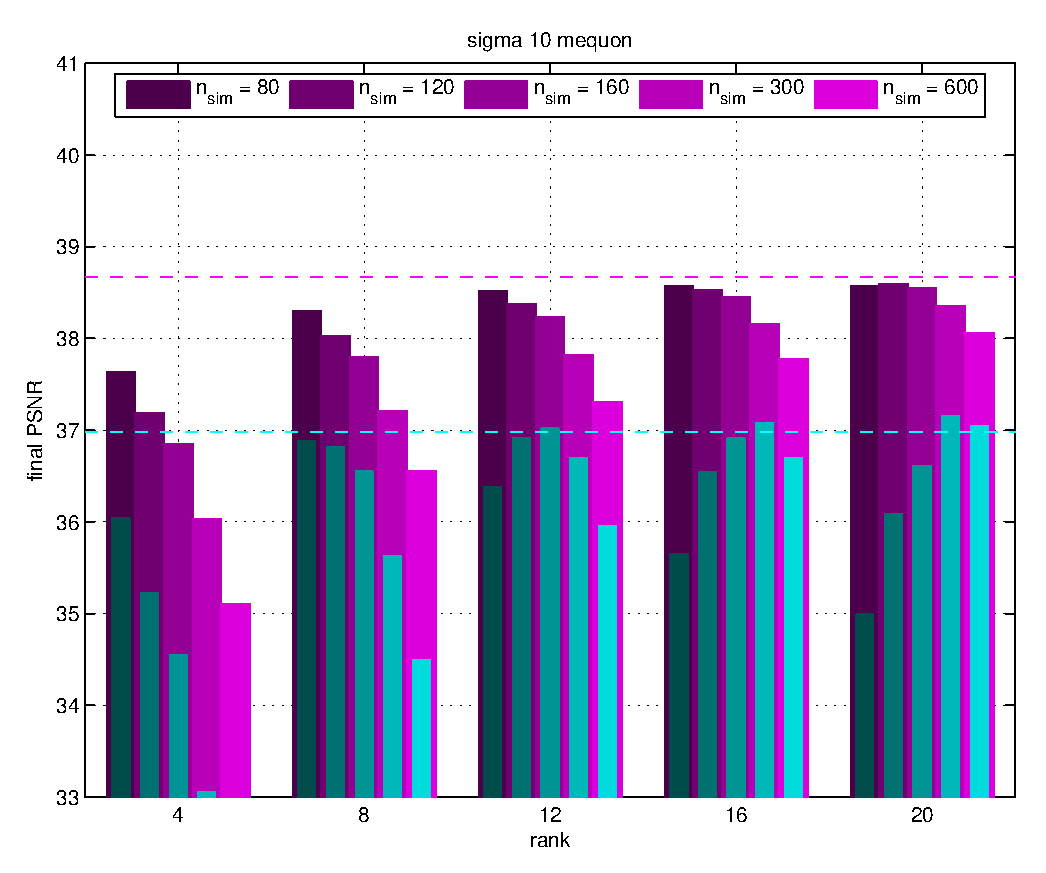
\includegraphics[width=.33\textwidth]{psnr_r1-np1-bars_s10_mequon.eps}%
		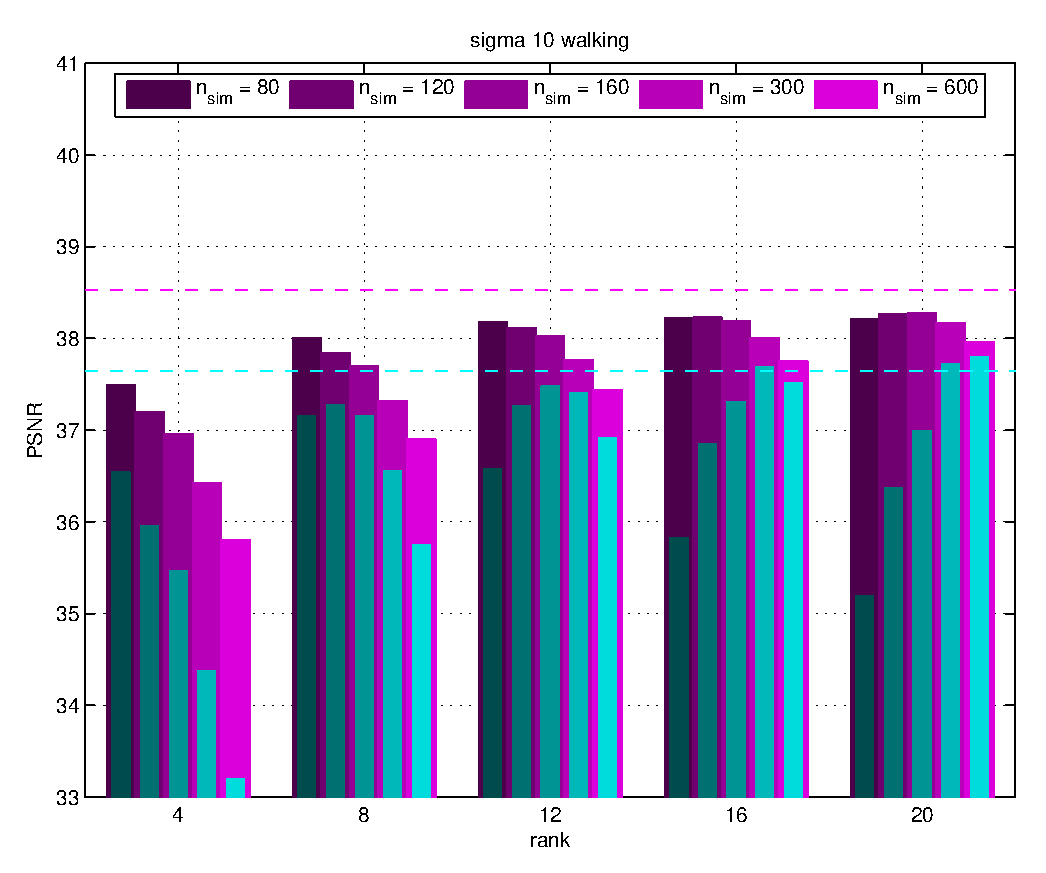
\includegraphics[width=.33\textwidth]{psnr_r1-np1-bars_s10_walking.eps}
	\end{center}

\end{frame}

\begin{frame}{PSNR tables - rank vs. number of patches, stage 1}

	\begin{center}
		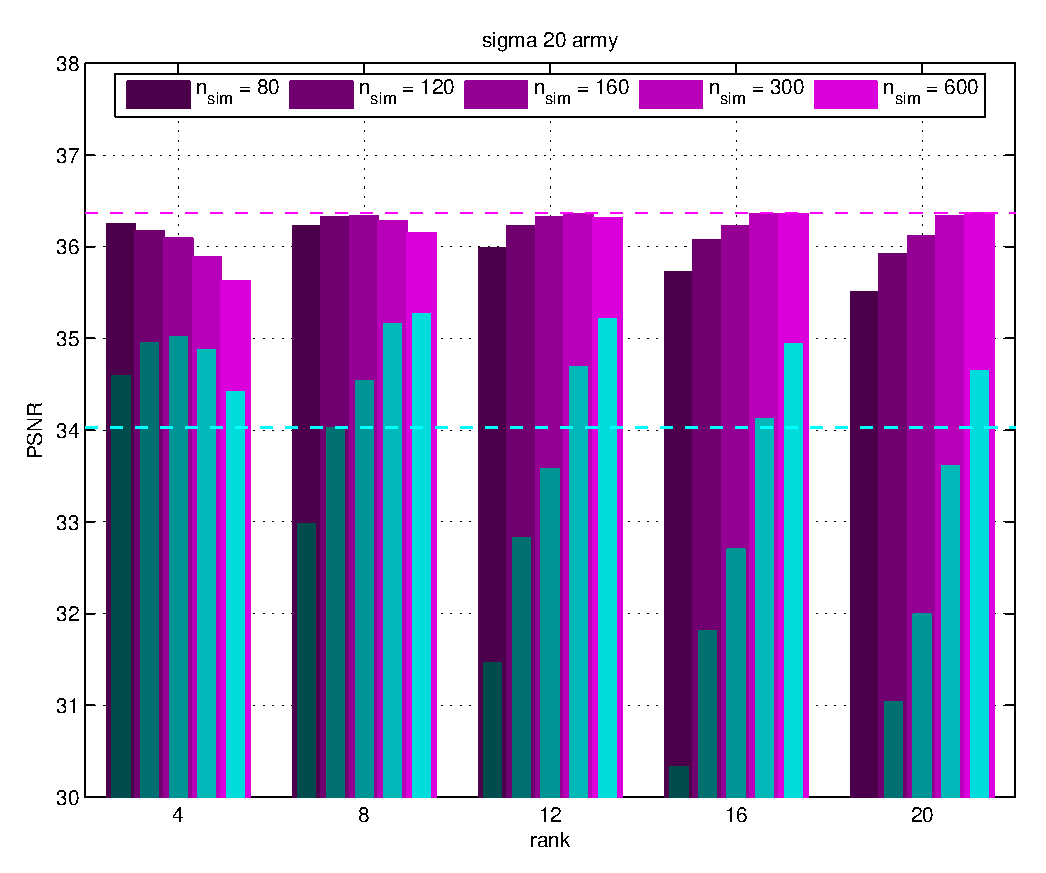
\includegraphics[width=.33\textwidth]{psnr_r1-np1-bars_s20_army.eps}%
		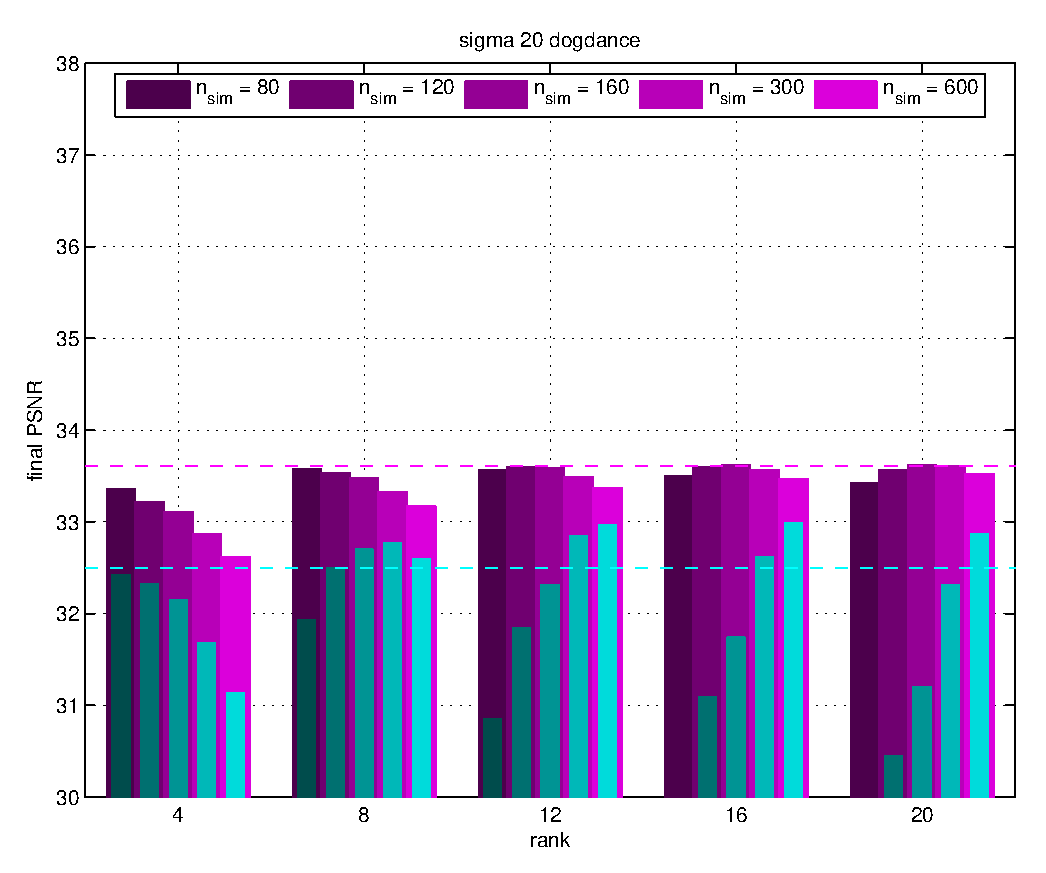
\includegraphics[width=.33\textwidth]{psnr_r1-np1-bars_s20_dogdance.eps}%
		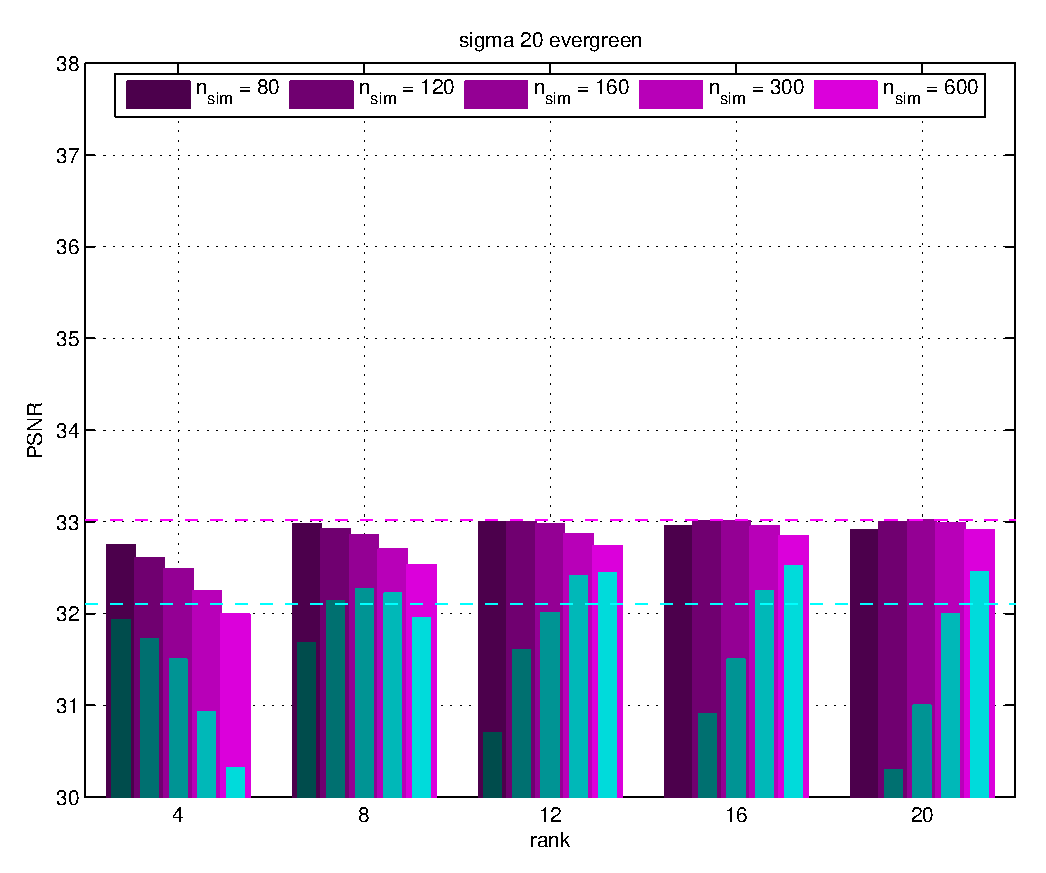
\includegraphics[width=.33\textwidth]{psnr_r1-np1-bars_s20_evergreen.eps}\\
		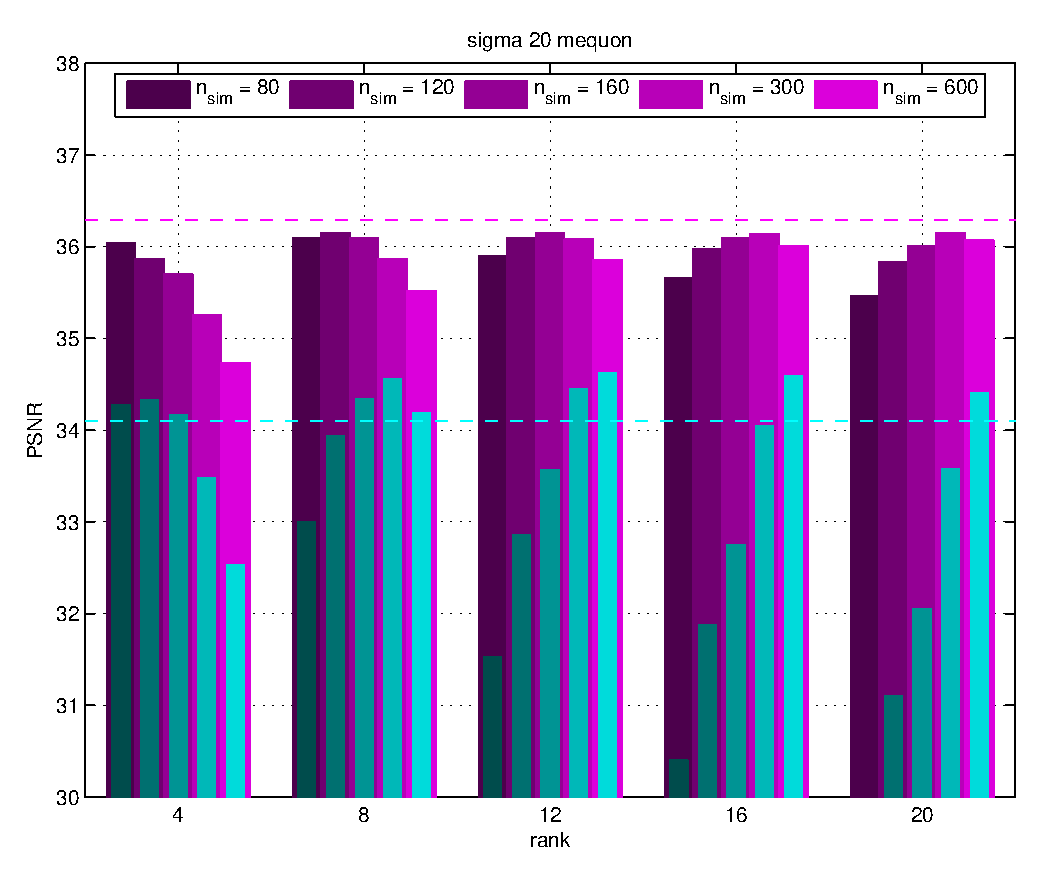
\includegraphics[width=.33\textwidth]{psnr_r1-np1-bars_s20_mequon.eps}%
		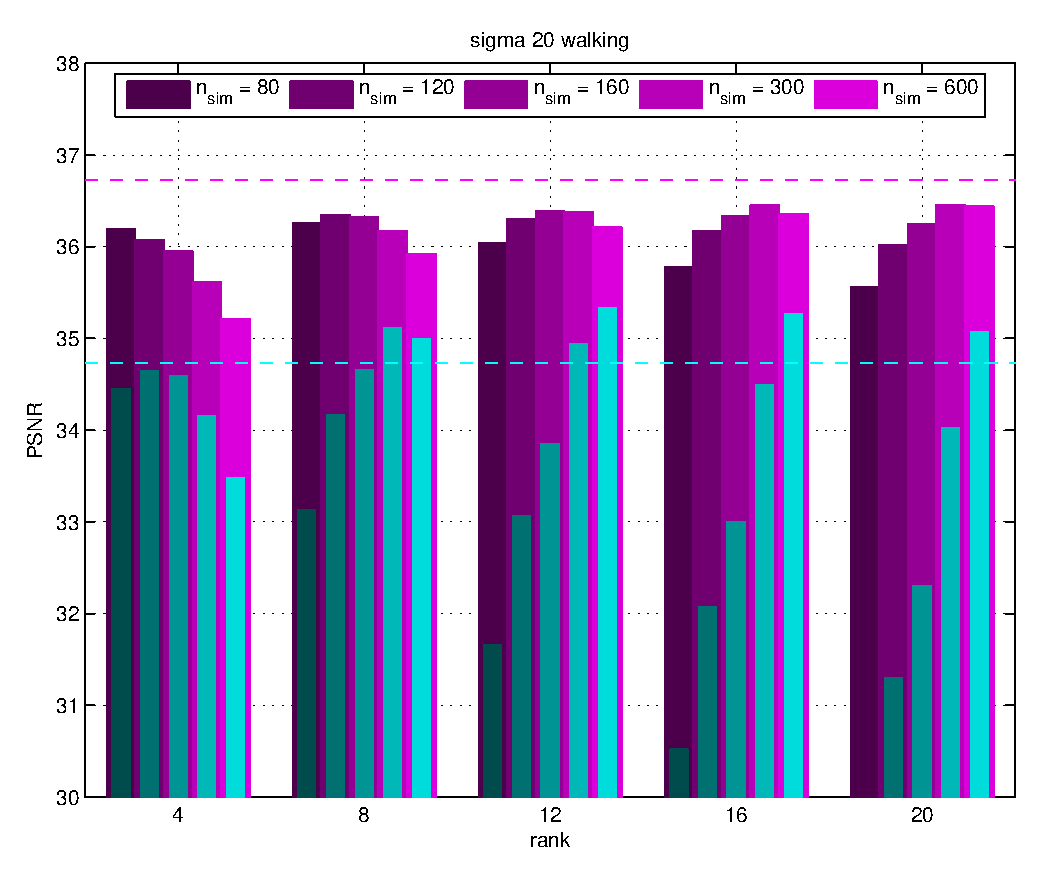
\includegraphics[width=.33\textwidth]{psnr_r1-np1-bars_s20_walking.eps}
	\end{center}

\end{frame}

\begin{frame}{PSNR tables - rank vs. number of patches, stage 1}

	\begin{center}
		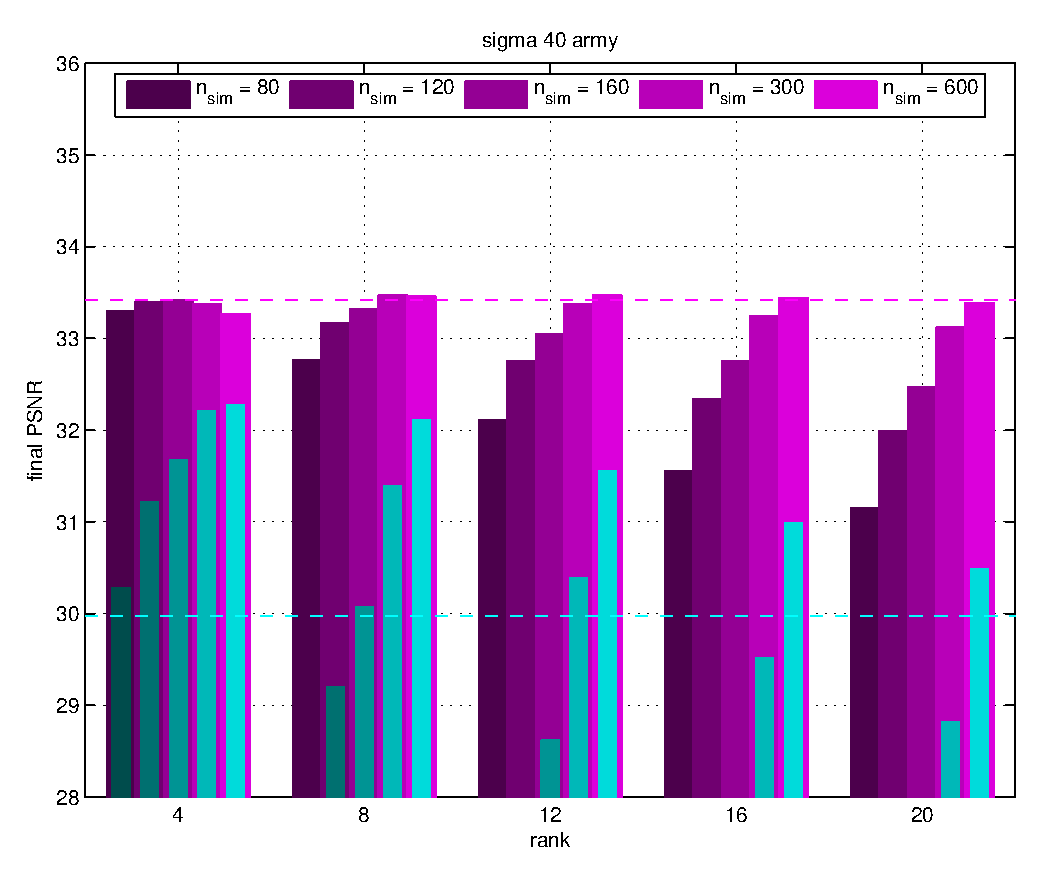
\includegraphics[width=.33\textwidth]{psnr_r1-np1-bars_s40_army.eps}%
		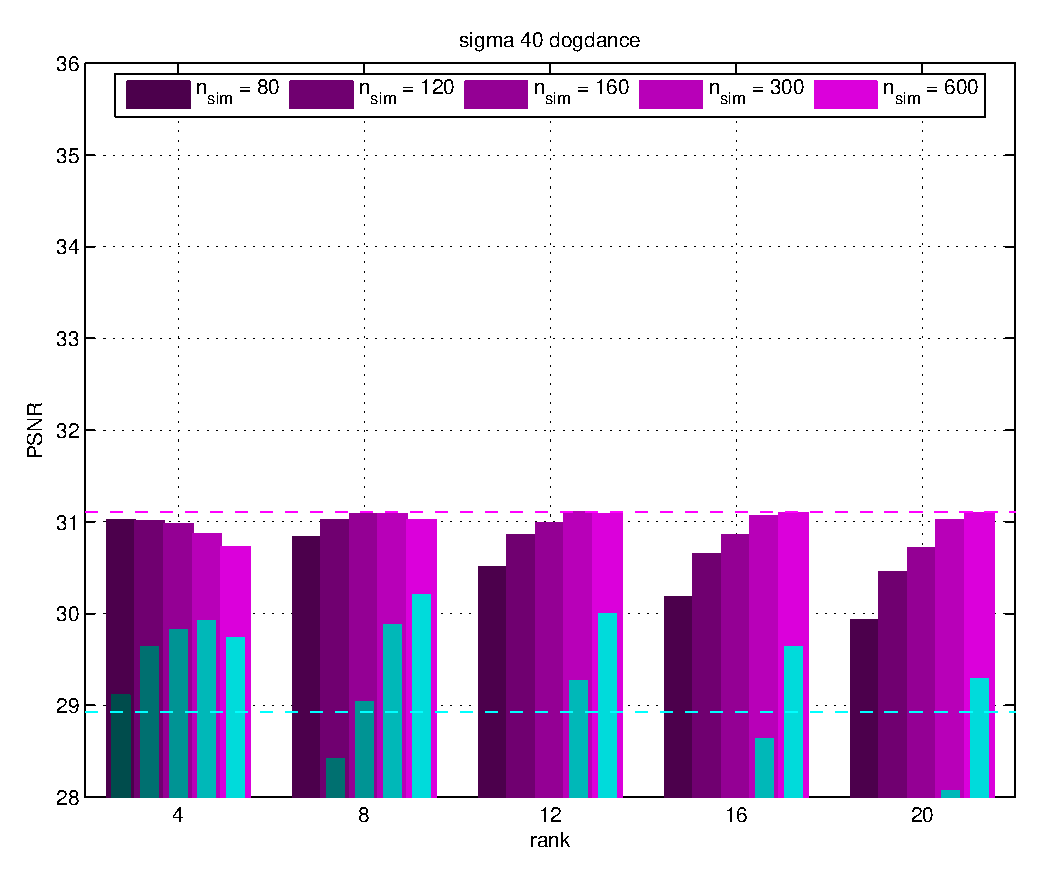
\includegraphics[width=.33\textwidth]{psnr_r1-np1-bars_s40_dogdance.eps}%
		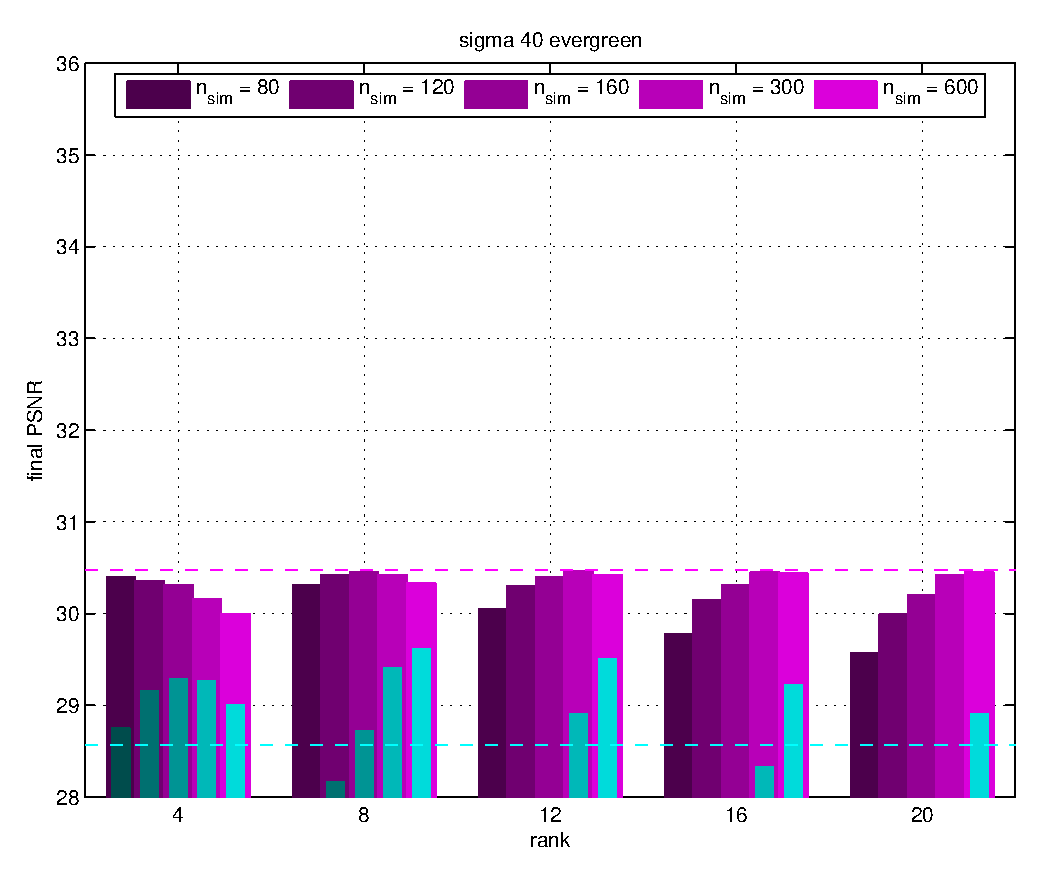
\includegraphics[width=.33\textwidth]{psnr_r1-np1-bars_s40_evergreen.eps}\\
		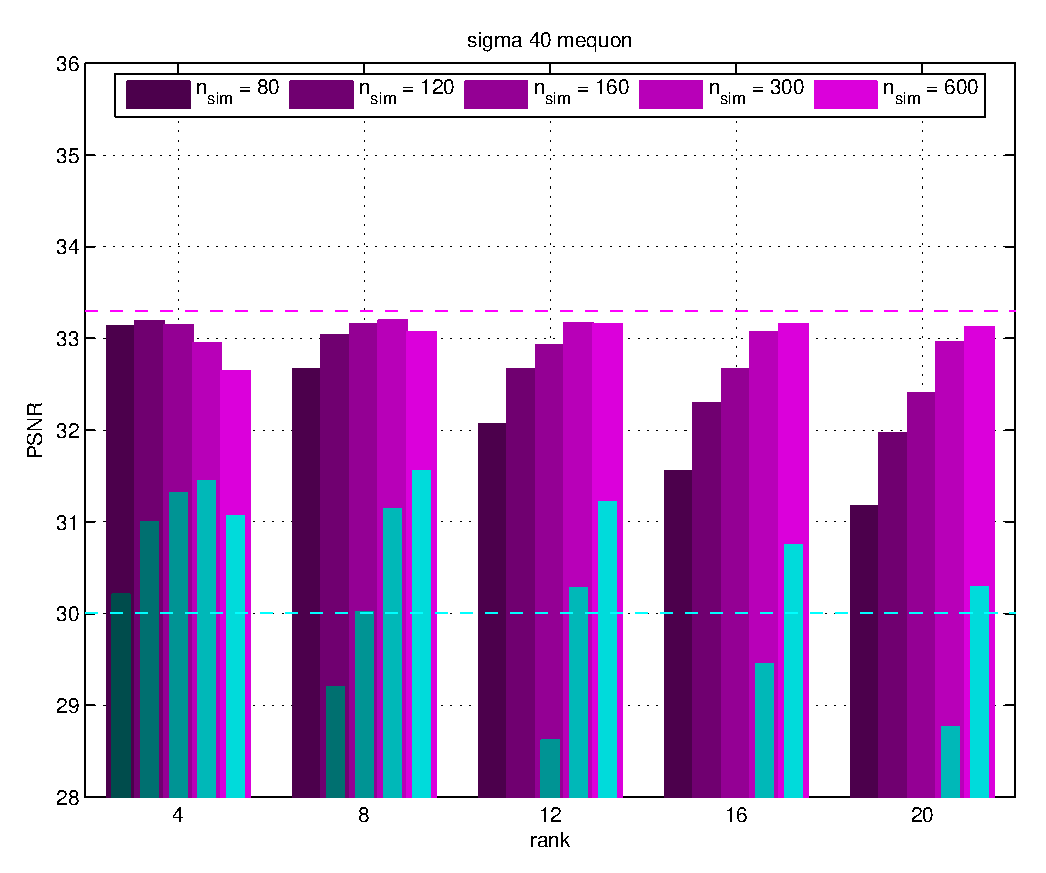
\includegraphics[width=.33\textwidth]{psnr_r1-np1-bars_s40_mequon.eps}%
		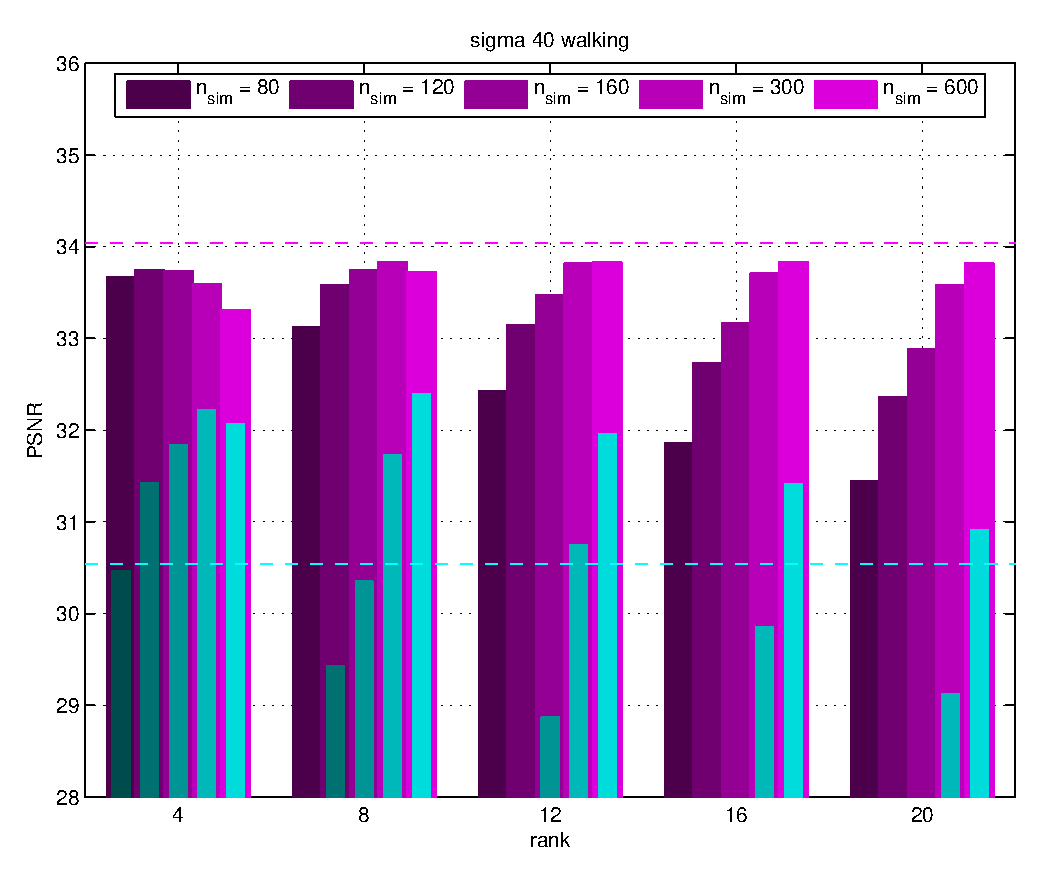
\includegraphics[width=.33\textwidth]{psnr_r1-np1-bars_s40_walking.eps}
	\end{center}

\end{frame}
\restoreframe

\multipleframe
\begin{frame}{Running time tables - rank vs. number of patches, stage 1}

	\begin{center}
		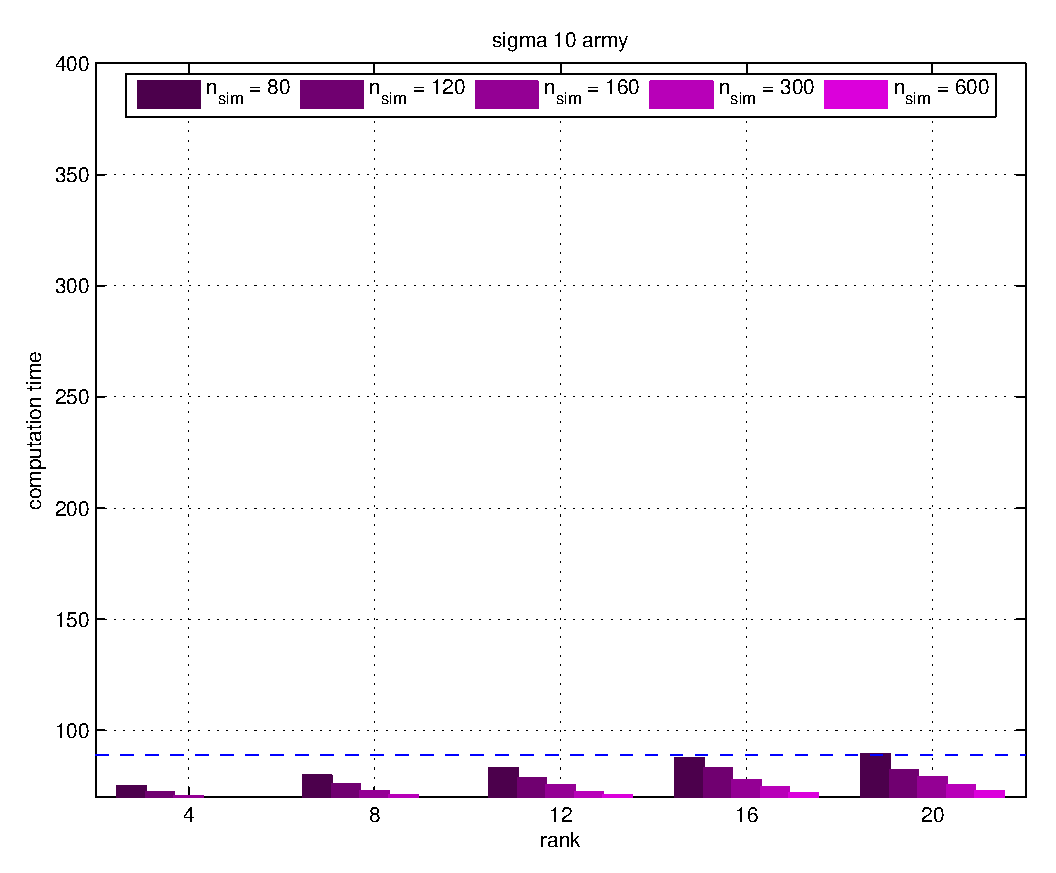
\includegraphics[width=.33\textwidth]{time_r1-np1-bars_s10_army.eps}%
		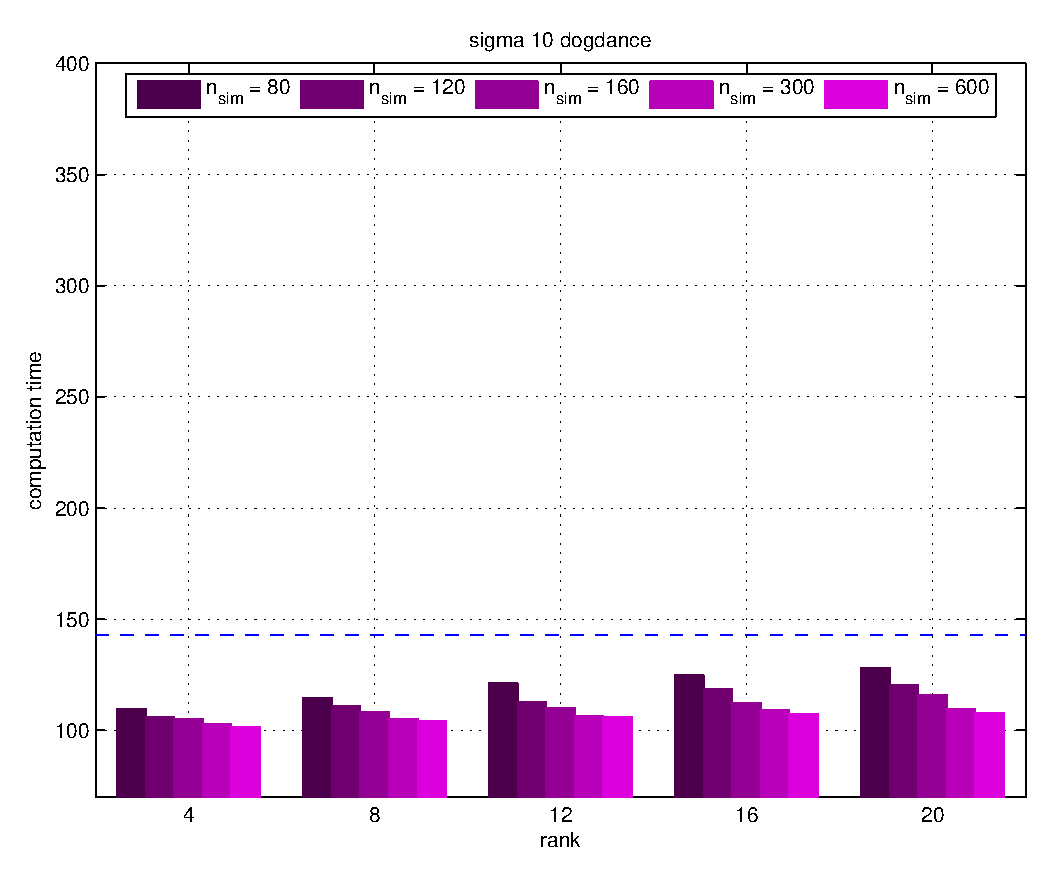
\includegraphics[width=.33\textwidth]{time_r1-np1-bars_s10_dogdance.eps}%
		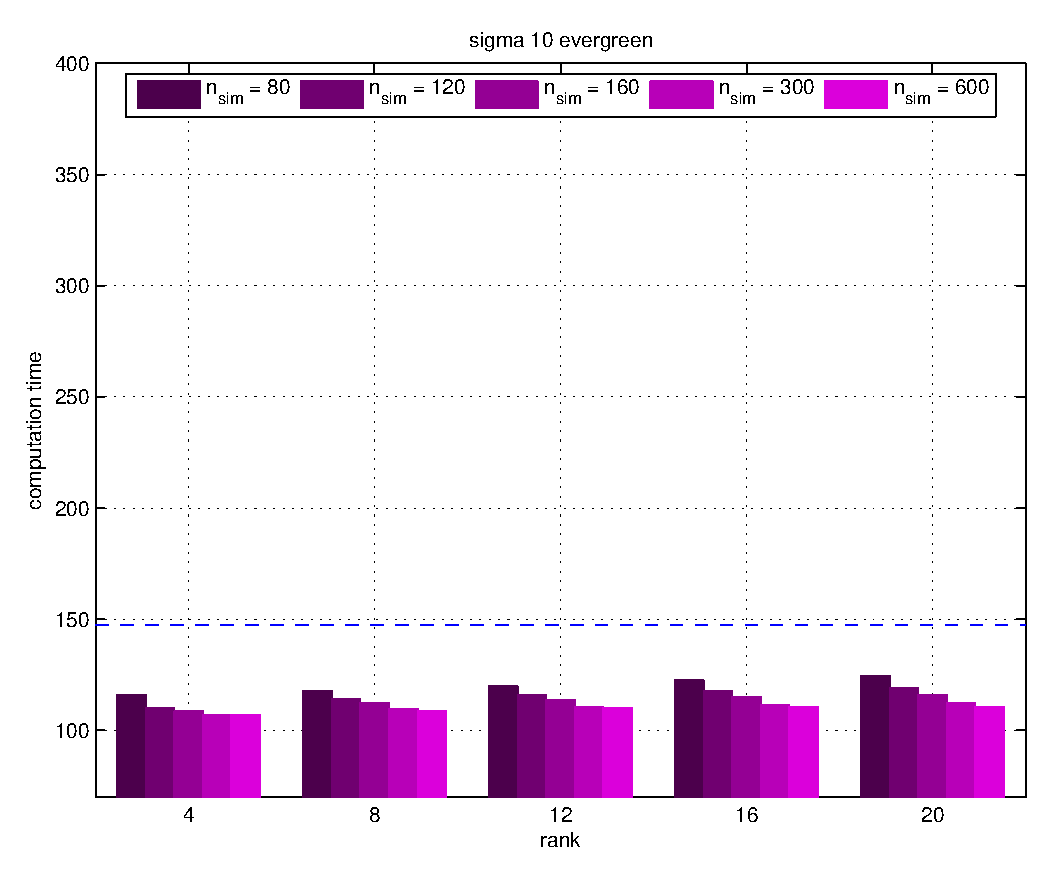
\includegraphics[width=.33\textwidth]{time_r1-np1-bars_s10_evergreen.eps}\\
		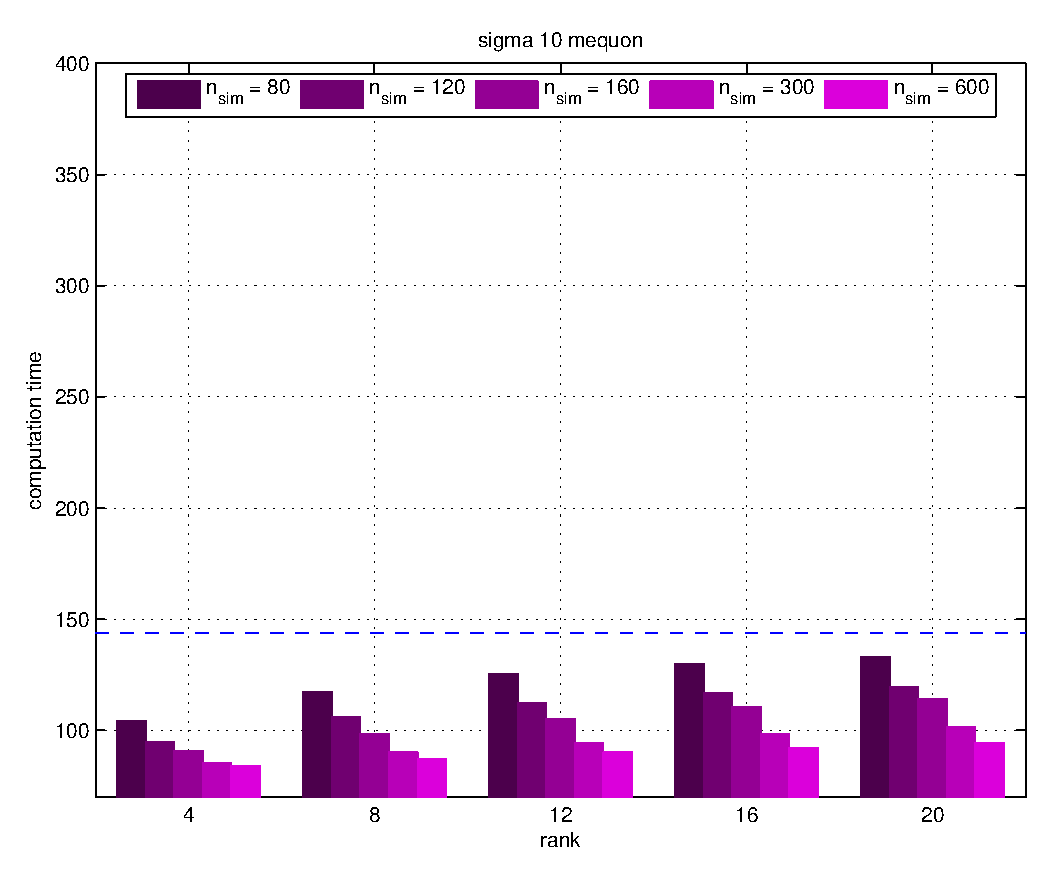
\includegraphics[width=.33\textwidth]{time_r1-np1-bars_s10_mequon.eps}%
		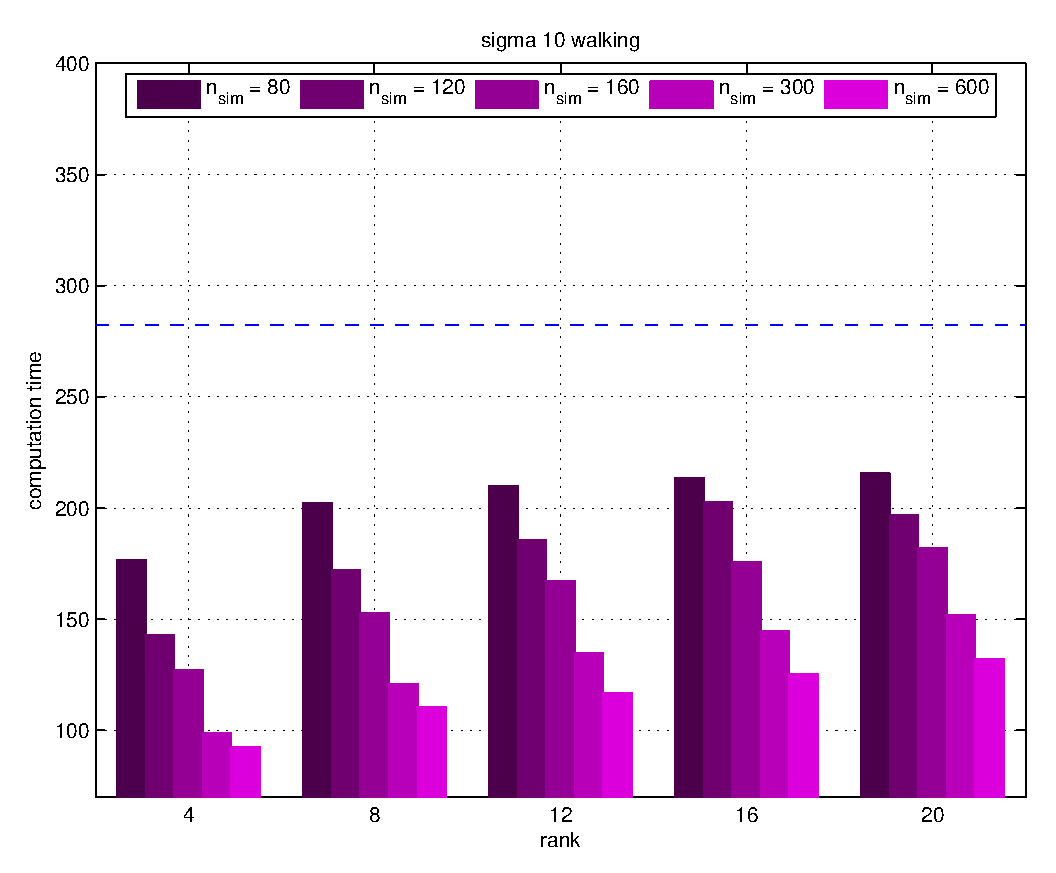
\includegraphics[width=.33\textwidth]{time_r1-np1-bars_s10_walking.eps}
	\end{center}

\end{frame}

\begin{frame}{Running time tables - rank vs. number of patches, stage 1}

	\begin{center}
		\includegraphics[width=.33\textwidth]{time_r1-np1-bars_s20_army.eps}%
		\includegraphics[width=.33\textwidth]{time_r1-np1-bars_s20_dogdance.eps}%
		\includegraphics[width=.33\textwidth]{time_r1-np1-bars_s20_evergreen.eps}\\
		\includegraphics[width=.33\textwidth]{time_r1-np1-bars_s20_mequon.eps}%
		\includegraphics[width=.33\textwidth]{time_r1-np1-bars_s20_walking.eps}
	\end{center}

\end{frame}

\begin{frame}{Running time tables - rank vs. number of patches, stage 1}

	\begin{center}
		\includegraphics[width=.33\textwidth]{time_r1-np1-bars_s40_army.eps}%
		\includegraphics[width=.33\textwidth]{time_r1-np1-bars_s40_dogdance.eps}%
		\includegraphics[width=.33\textwidth]{time_r1-np1-bars_s40_evergreen.eps}\\
		\includegraphics[width=.33\textwidth]{time_r1-np1-bars_s40_mequon.eps}%
		\includegraphics[width=.33\textwidth]{time_r1-np1-bars_s40_walking.eps}
	\end{center}

\end{frame}

\begin{frame}{Conclusions - rank vs. number of patches, stage 1}
	\begin{itemize}\itemsep=2cm
		\item We can improve the basic estimate, but we cannot improve the final estimate.
		\item The qualitative behaviour depends on the noise level.
	\end{itemize}
\end{frame}

\begin{frame}{Conclusions - rank vs. number of patches, stage 1}
	For $\sigma = 40$:
	\begin{itemize}\itemsep=.3cm
		\item The basic and final PSNRs increase with $n_{\text{sim}}$.
		\item For a fixed $n_{\text{sim}}$, the basic PSRN incease when the
			rank decreases until $r = 8$, \textbf{but the final PSNR does not change!}
		\item The basic estimate can improve substantially w.r.t. to the
			full rank reference, but the final estimate cannot be improved.
		\item Best basic results seem to be obtained with $n_{\text{sim}} = 
			600$ and $r = 8$.
		\item Best final results seem to be obtained with $n_{\text{sim}}\in
			[300,600]$ and $r > 8$.
	\end{itemize}
\end{frame}

\begin{frame}{Conclusions - rank vs. number of patches, stage 1}
	For $\sigma = 20$:
	\begin{itemize}\itemsep=.3cm
		\item Excluding $n_{\text{sim}} = 600$, for a fixed
			$n_{\text{sim}}$, the basic PSRN inceases when the rank decreases
			until $r = 8$ (and until $r = 12$ for $n_{\text{sim}} = 300$.
			The final PSNR does not have a clear behaviour.
		\item For fixed $r > 8$, increasing $n_{\text{sim}}$ is beneficial for the
			basic estimate, but not for the final estimate.
		\item The basic estimate can improve w.r.t. to the
			full rank reference, but the final estimate cannot be improved.
		\item Best basic results seem to be obtained with $n_{\text{sim}} = 
			600$ and $r = 12$.
		\item Best final results seem to be obtained with $n_{\text{sim}}=
			160$ and $r = 12$, or $n_{\text{sim}}=
			300$ and $r = 16$.
	\end{itemize}
\end{frame}

\begin{frame}{Conclusions - rank vs. number of patches, stage 1}
	For $\sigma = 10$:
	\begin{itemize}\itemsep=.3cm
		\item Since the data has more details, one cannot model large sets of patches
			with low rank covariances as before. Increasing $n_{\text{sim}}$ now can drops
			the quality, and this happens earlier the lower the rank.
		\item For a fixed $n_{\text{sim}}$, decreasing the rank does not
			improve the basic PSRN any more.
		\item The basic and final estimates have opposing behaviours w.r.t. $n_{\text{sim}}$.
		\item Best basic results seem to be obtained with $n_{\text{sim}} > 
			160$ and $r > 8$.
		\item Best final results seem to be obtained with $n_{\text{sim}}<
			300$ and $r > 4$.
	\end{itemize}
\end{frame}

\begin{frame}{Conclusions - rank vs. number of patches, stage 1}
	Based on this observations, we propose the following parameters:
	\[r = 160\quad\quad n_{\text{sim}} = \max(15\sigma,cr).\]

	Notes:
	\begin{itemize}\itemsep=.3cm
		\item The rank $r$ could be smaller, but there is not much difference in
			computational time nor in PSNR. We therefore choose a more
			conservative higher rank.
		\item The linear relation $n_{\text{sim}} = 15\sigma$ comes from observing that
			for good results are obtained at
			\begin{center}
				\begin{tabular}{l | c c c}
					$\sigma$         &  10 &  20 &  40 \\ 
					$n_{\text{sim}}$ & 150 & 300 & 600 
				\end{tabular}
			\end{center}
		\item $c\geqslant1$ is a constant multiplying the rank. When $15\sigma$
			is too small, we ignore the linear relation and take a fixed number of
			patches which depend on the rank. \textbf{We should do more experiments
			to determine an appropriate value for $c$. For the moment, we will choose
         5.} With this choice,
			\[
				n_{\text{sim}} =
				\left\{
				\begin{array}{l l}
					15\sigma & \text{if }\sigma \geqslant r/3\\
					5r       & \text{if }\sigma < r/3
				\end{array}
				\right.
			\]
			For $r = 16$, $5r = 80$ and $r/3 \approx 5.33$.
	\end{itemize}
\end{frame}


\restoreframe

\end{document}

